% ******************************* PhD Thesis Template **************************
% Please have a look at the README.md file for info on how to use the template

% LP added "ONESIDE" or "OPENANY" to remove blank pages
\documentclass[a4paper,12pt,oneside,times,authoryear,print,chapter]{Classes/PhDThesisPSnPDF}

% ******************************************************************************
% ******************************* Class Options ********************************
% *********************** See README for more details **************************
% ******************************************************************************

% `a4paper'(The University of Cambridge PhD thesis guidelines recommends a page
% size a4 - default option) or `a5paper': A5 Paper size is also allowed as per
% the Cambridge University Engineering Deparment guidelines for PhD thesis
%
% `11pt' or `12pt'(default): Font Size 10pt is NOT recommended by the University
% guidelines
%
% `oneside' or `twoside'(default): Printing double side (twoside) or single
% side.
%
% `print': Use `print' for print version with appropriate margins and page
% layout. Leaving the options field blank will activate Online version.
%
% `index': For index at the end of the thesis
%
% `draftclassic': For draft mode without loading any images (same as draft in book)
%
% `draft': Special draft mode with line numbers, images, and water mark with
% timestamp and custom text. Position of the text can also be modified.
%
% `abstract': To generate only the title page and abstract page with
% dissertation title and name, to submit to the Student Registry
%
% `chapter`: This option enables only the specified chapter and it's references
%  Useful for review and corrections.
%
% ************************* Custom Page Margins ********************************
%
% `custommargin`: Use `custommargin' in options to activate custom page margins,
% which can be defined in the preamble.tex. Custom margin will override
% print/online margin setup.
%
% *********************** Choosing the Fonts in Class Options ******************
%
% `times' : Times font with math support. (The Cambridge University guidelines
% recommend using times)
%
% `fourier': Utopia Font with Fourier Math font (Font has to be installed)
%            It's a free font.
%
% `customfont': Use `customfont' option in the document class and load the
% package in the preamble.tex
%
% default or leave empty: `Latin Modern' font will be loaded.
%
% ********************** Choosing the Bibliography style ***********************
%
% `authoryear': For author-year citation eg., Krishna (2013)
%
% `numbered': (Default Option) For numbered and sorted citation e.g., [1,5,2]
%
% `custombib': Define your own bibliography style in the `preamble.tex' file.
%              `\RequirePackage[square, sort, numbers, authoryear]{natbib}'.
%              This can be also used to load biblatex instead of natbib
%              (See Preamble)
%
% **************************** Choosing the Page Style *************************
%
% `default (leave empty)': For Page Numbers in Header (Left Even, Right Odd) and
% Chapter Name in Header (Right Even) and Section Name (Left Odd). Blank Footer.
%
% `PageStyleI': Chapter Name next & Page Number on Even Side (Left Even).
% Section Name & Page Number in Header on Odd Side (Right Odd). Footer is empty.
%
% `PageStyleII': Chapter Name on Even Side (Left Even) in Header. Section Number
% and Section Name in Header on Odd Side (Right Odd). Page numbering in footer

% Uncomment to change page style


% \pagestyle{PageStyleII}
% Preamble: Contains packages and user-defined commands and settings
% ******************************************************************************
% ****************************** Custom Margin *********************************

% Add `custommargin' in the document class options to use this section
% Set {innerside margin / outerside margin / topmargin / bottom margin}  and
% other page dimensions
\ifsetCustomMargin
  \RequirePackage[left=37mm,right=30mm,top=35mm,bottom=30mm]{geometry}
  \setFancyHdr % To apply fancy header after geometry package is loaded
\fi

% Add spaces between paragraphs
%\setlength{\parskip}{0.5em}
% Ragged bottom avoids extra whitespaces between paragraphs
\raggedbottom
% To remove the excess top spacing for enumeration, list and description
%\usepackage{enumitem}
%\setlist[enumerate,itemize,description]{topsep=0em}

% *****************************************************************************
% ******************* Fonts (like different typewriter fonts etc.)*************

% Add `customfont' in the document class option to use this section

\ifsetCustomFont
  % Set your custom font here and use `customfont' in options. Leave empty to
  % load computer modern font (default LaTeX font).
  %\RequirePackage{helvet}

  % For use with XeLaTeX
  %  \setmainfont[
  %    Path              = ./libertine/opentype/,
  %    Extension         = .otf,
  %    UprightFont = LinLibertine_R,
  %    BoldFont = LinLibertine_RZ, % Linux Libertine O Regular Semibold
  %    ItalicFont = LinLibertine_RI,
  %    BoldItalicFont = LinLibertine_RZI, % Linux Libertine O Regular Semibold Italic
  %  ]
  %  {libertine}
  %  % load font from system font
  %  \newfontfamily\libertinesystemfont{Linux Libertine O}
\fi

% *****************************************************************************
% **************************** Custom Packages ********************************

% ************************* Algorithms and Pseudocode **************************

%\usepackage{algpseudocode}


% ********************Captions and Hyperreferencing / URL **********************

% Captions: This makes captions of figures use a boldfaced small font.
%\RequirePackage[small,bf]{caption}

\RequirePackage[labelsep=space,tableposition=top]{caption}
\renewcommand{\figurename}{Fig.} %to support older versions of captions.sty


% *************************** Graphics and figures *****************************

%\usepackage{rotating}
%\usepackage{wrapfig}

% Uncomment the following two lines to force Latex to place the figure.
% Use [H] when including graphics. Note 'H' instead of 'h'
%\usepackage{float}
%\restylefloat{figure}

% Subcaption package is also available in the sty folder you can use that by
% uncommenting the following line
% This is for people stuck with older versions of texlive
%\usepackage{sty/caption/subcaption}
\usepackage{subcaption}
% ********************************** Tables ************************************
\usepackage{booktabs} % For professional looking tables
\usepackage{multirow}

%\usepackage{multicol}
%\usepackage{longtable}
%\usepackage{tabularx}


% *********************************** SI Units *********************************
\usepackage{siunitx} % use this package module for SI units


% ******************************* Line Spacing *********************************

% Choose linespacing as appropriate. Default is one-half line spacing as per the
% University guidelines

 \doublespacing
%\onehalfspacing
% \singlespacing


% ************************ Formatting / Footnote *******************************

% Don't break enumeration (etc.) across pages in an ugly manner (default 10000)
%\clubpenalty=500
%\widowpenalty=500

%\usepackage[perpage]{footmisc} %Range of footnote options


% *****************************************************************************
% *************************** Bibliography  and References ********************

%\usepackage{cleveref} %Referencing without need to explicitly state fig /table

% Add `custombib' in the document class option to use this section
\ifuseCustomBib
   \RequirePackage[round, sort, numbers, authoryear]{natbib} % CustomBib

% If you would like to use biblatex for your reference management, as opposed to the default `natbibpackage` pass the option `custombib` in the document class. Comment out the previous line to make sure you don't load the natbib package. Uncomment the following lines and specify the location of references.bib file

%\RequirePackage[backend=biber, style=numeric-comp, citestyle=numeric, sorting=nty, natbib=true]{biblatex}
%\bibliography{References/references} %Location of references.bib only for biblatex

\fi

% changes the default name `Bibliography` -> `References'
\renewcommand{\bibname}{References}


% ******************************************************************************
% ************************* User Defined Commands ******************************
% ******************************************************************************

% *********** To change the name of Table of Contents / LOF and LOT ************

% \renewcommand{\contentsname}{My Table of Contents}
% \renewcommand{\listfigurename}{My List of Figures}
% \renewcommand{\listtablename}{My List of Tables}
% \renewcommand{\listalgorithmcfnamename}{My List of Algorithms}

% ********************** TOC depth and numbering depth *************************

\setcounter{secnumdepth}{4}
\setcounter{tocdepth}{2}


% ******************************* Nomenclature *********************************

% To change the name of the Nomenclature section, uncomment the following line

%\renewcommand{\nomname}{Symbols}


% ********************************* Appendix ***********************************

% The default value of both \appendixtocname and \appendixpagename is `Appendices'. These names can all be changed via:

\renewcommand{\appendixtocname}{List of appendices}
\renewcommand{\appendixname}{Appndx}

% *********************** Configure Draft Mode **********************************

% Uncomment to disable figures in `draft'
%\setkeys{Gin}{draft=true}  % set draft to false to enable figures in `draft'

% These options are active only during the draft mode
% Default text is "Draft"
%\SetDraftText{DRAFT}

% Default Watermark location is top. Location (top/bottom)
%\SetDraftWMPosition{bottom}

% Draft Version - default is v1.0
%\SetDraftVersion{v1.1}

% Draft Text grayscale value (should be between 0-black and 1-white)
% Default value is 0.75
%\SetDraftGrayScale{0.8}


% ******************************** Todo Notes **********************************
%% Uncomment the following lines to have todonotes.

%\ifsetDraft
%	\usepackage[colorinlistoftodos]{todonotes}
%	\newcommand{\mynote}[1]{\todo[author=kks32,size=\small,inline,color=green!40]{#1}}
%\else
%	\newcommand{\mynote}[1]{}
%	\newcommand{\listoftodos}{}
%\fi

% Example todo: \mynote{Hey! I have a note}

\usepackage{enumitem}
\usepackage{titlesec}

\usepackage{graphicx}
% \usepackage[scale=1]{geometry}
% \usepackage{pdfpages}

\usepackage{amsmath}

\usepackage[ruled,vlined,linesnumbered,algochapter]{algorithm2e}
\usepackage{algpseudocode}
\usepackage{array}

%class diagrams
\usepackage{tikz}
\usepackage[simplified]{pgf-umlcd}

\usepackage{multirow}

\usepackage{svg}


% ************************ Thesis Information & Meta-data **********************
% Thesis title and author information, refernce file for biblatex
%% ************************ Thesis Information & Meta-data **********************
%% The title of the thesis
\title{Cancelable biometrics using hand geometry-based steganographic techniques}
%\texorpdfstring is used for PDF metadata. Usage:
%\texorpdfstring{LaTeX_Version}{PDF Version (non-latex)} eg.,
%\texorpdfstring{$sigma$}{sigma}

%% Subtitle (Optional)
%\subtitle{No Subtitle}

%% The full name of the author
\author{Louis-Philip Shahim}

%% Department (eg. Department of Engineering, Maths, Physics)
\dept{Department of Natural Sciences}

%% University and Crest
\university{North West University, Potchefstroom}
% Crest minimum should be 30mm.
%\crest{
\includegraphics[width=0.2\textwidth]{University_Crest}}
%% Use this crest, if you are using the college crest
%% Crest long miminum should be 65mm
%\crest{\includegraphics[width=0.45\textwidth]{logo}}

%% College shield [optional] 
% Crest minimum should be 30mm.
%\collegeshield{\includegraphics[width=0.2\textwidth]{CollegeShields/nwu_logo}}


%% Supervisor (optional)
%% for multiple supervisors, append each supervisor with the \newline command
   \supervisor{D.P. Snyman \newline}

%% Supervisor Role (optional) - Supervisor (default) or advisor
% \supervisorrole{\textbf{Supervisors: }}
%% if no title is desired:
% \supervisorrole{}

%% Supervisor line width: required to align supervisors
%\supervisorlinewidth{0.35\textwidth}

%% Advisor (optional)
%% for multiple advisors, append each advisor with the \newline command
%\advisor{Dr. A. Advisor\newline
%Dr. B. Advisor}
     
%% Advisor Role (optional) - Advisor (default) or leave empty
% \advisorrole{Advisors: }
%% if no title is required
% \advisorrole{}

%% Advisor line width: required to align supervisors
%\advisorlinewidth{0.25\textwidth}


%% You can redefine the submission text:
% Default as per the University guidelines:
% ``This dissertation is submitted for the degree of''
%\renewcommand{\submissiontext}{change the default text here if needed}

%% Full title of the Degree
\degreetitle{Master of Computer Science and Information Systems}

%% College affiliation (optional)
\college{NWU}

%% Submission date
% Default is set as {\monthname[\the\month]\space\the\year}
\degreedate{November 2018} 

%% Meta information
%\subject{LaTeX} \keywords{{LaTeX} {PhD Thesis} {Engineering} {University of Cambridge}}



% ***************************** Abstract Separate ******************************
% To printout only the titlepage and the abstract with the PhD title and the
% author name for submission to the Student Registry, use the `abstract' option in
% the document class.

% \ifdefineAbstract
%  \pagestyle{empty}
%  \includeonly{Declaration/declaration, Abstract/abstract}
% \fi

% ***************************** Chapter Mode ***********************************
% The chapter mode allows user to only print particular chapters with references
% Title, Contents, Frontmatter are disabled by default
% Useful option to review a particular chapter or to send it to supervisior.
% To use choose `chapter' option in the document class

 \ifdefineChapter
 	\includeonly{Chapter1/chapter1}
%  	\includeonly{Chapter2/chapter2}
%  	\includeonly{Chapter3/chapter3}
%  	\includeonly{Chapter4/chapter4}
%  	\includeonly{Chapter5/chapter5}
 \fi

\usepackage{pdfpages}
% ******************************** Front Matter ********************************
\begin{document}
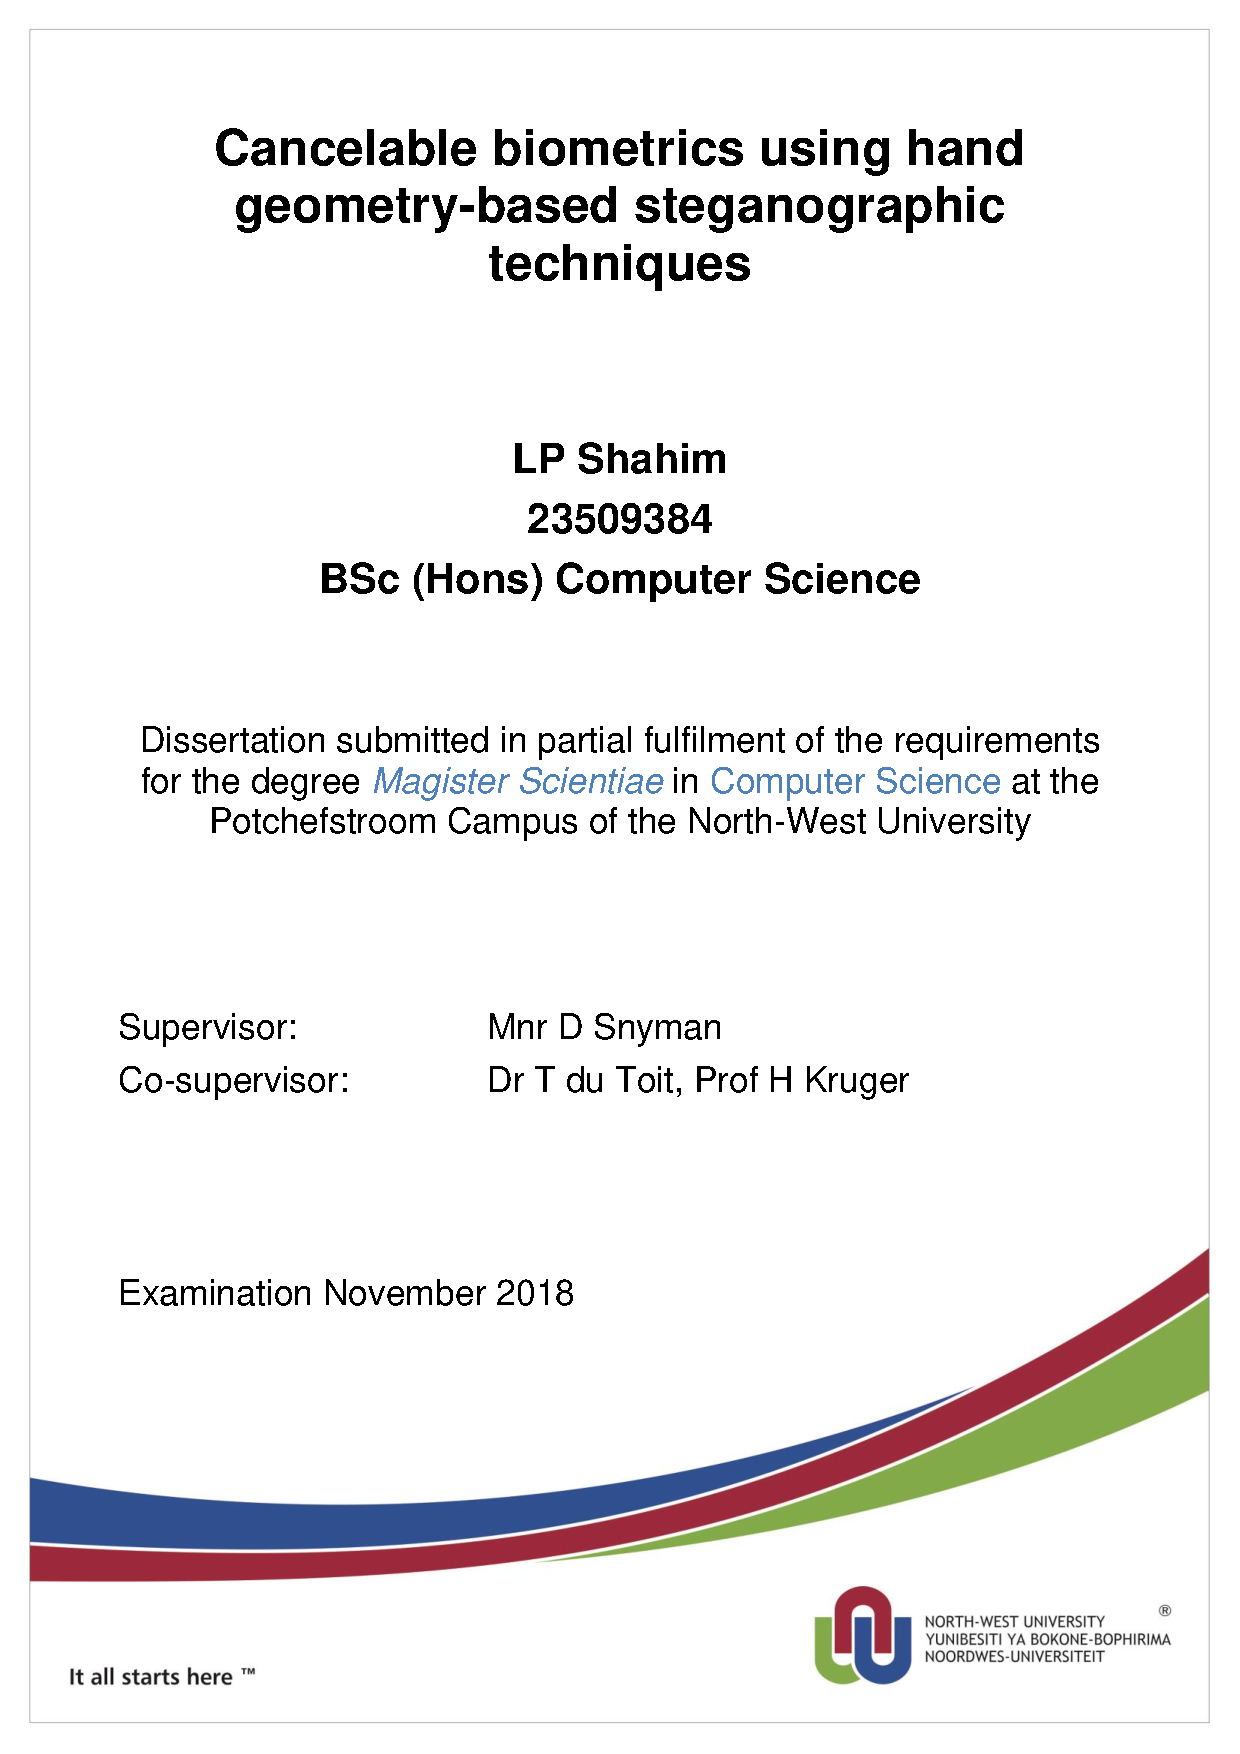
\includepdf{CoverPage.pdf}
\frontmatter

% \maketitle

% ******************************* Thesis Dedidcation ********************************

\begin{dedication} 

\begin{displayquote}
"Make your parents proud, your enemies jealous and yourself happy." - Anon
\end{displayquote}
I would like to dedicate this dissertation to my loving parents and wonderful sister. Without all of you, this would not have been possible. I am extremely blessed to have been given this opportunity. \\
To my late grandfather, and my namesake, I know you are looking down at me and smiling. Thank you for all of your love and support. I would have loved to celebrate this accomplishment with you over a whisky.\\ 
Lastly, to my Lord God Almighty for the continuous blessings, protection and guidance bestowed upon me. I am eternally grateful.\\


\end{dedication}


% ******************************* Thesis Declaration ***************************

\begin{declaration}

I hereby declare that except where specific reference is made to the work of 
others, the contents of this dissertation are original and have not been 
submitted in whole or in part for consideration for any other degree or 
qualification in this, or any other university. This dissertation is my own 
work and contains nothing which is the outcome of work done in collaboration 
with others, except as specified in the text and Acknowledgements. This 
dissertation contains fewer than 65,000 words including appendices, 
bibliography, footnotes, tables and equations and has fewer than 150 figures.

% Author and date will be inserted automatically from thesis.tex \author \degreedate \\

\end{declaration}

% ************************** Thesis Acknowledgements **************************

\begin{acknowledgements}      


And I would like to acknowledge ...


\end{acknowledgements}

% ************************** Thesis Abstract *****************************
% Use `abstract' as an option in the document class to print only the titlepage and the abstract.
\begin{abstract}

Biometrics have long been used as an accepted user authentication method and have been
implemented as a security measure in many real-world systems including personal computers,
mobile devices, and physical access control. By encoding a person’s physical attributes the disadvantages of traditional password based security, like passwords being lost or stolen, can be overcome. One of the factors that hampers the acceptance of biometric authentication systems is that users have to submit private biometric data to the authentication systems and should these systems be compromised, a digital copy of their biometrics becomes available for exploitation.

The concept of Cancelable Biometrics has to do with obfuscating of biometric
information that is used for biometric authentication, whether the information is in storage
or in transit. This ensures that biometric information of a person cannot be reconstructed
when it is observed by a third party. With the use of a cancelling
technique, one can assure anonymity of users within the system and prevent unauthorised
usage of digitised biometric information.

The primary aim of this study was to develop a technique that ensures cancelability of biometrics
based on hand geometry information from a  Leap Motion Controller and steganographic storage techniques.
To achieve the primary aim, the following secondary objectives were addressed: i) Perform a literature study to discuss the use and implementation of cancelable biometrics, steganography, hand geometry authentication and the Leap Motion Controller. ii) Design and implementation of the system. iii) Evaluation of the created system using error-based metrics and iterative validation testing.

Based on the recommendations from literature, a biometric authentication system was designed and implemented which uses latent hand geometry information from a Leap Motion Controller to construct biometric templates. The cancelability of the biometric templates were ensured by implementing user-specific transforms to the templates and employing steganography techniques for a novel storage solution. The system's performance was evaluated both in terms of the various components that were integrated in the system, and in terms of its overall performance. Even though the Leap Motion Controller proved to be an effective an efficient biometric sensor, the use of hand geometry as the source of user biometrics in this context did not exhibit the required level of uniqueness. Given varying levels of tolerance that the system allows for, biometric authentication can still be performed, however, with a trade-off between the true acceptance and false acceptance rates. The negative effect of the tolerance levels were mitigated by introducing a user PIN as a second authentication factor.\\

\textbf{Key terms:}
CANCELABLE BIOMETRICS, INFORMATION SECURITY, LEAP MOTION CONTROLLER, MULTIFACTOR AUTHENTICATION, STEGANOGRAPHY, HAND GEOMETRY.

\newpage


\chapter*{\centering \Large Opsomming}

Biometrie word al vir 'n geruime tyd gebruik as 'n aanvaarde gebruikerverifikasiemetode en word geïmplementeer as 'n sekuriteitsmaatreël in baie regtewêreld stelsels, insluitende persoonlike rekenaars, mobiele toestelle en fisiese toegangsbeheer. Deur ʼn persoon se fisiese eienskappe te enkodeer kan die nadele van tradisionele wagwoordgebaseerde sekuriteit, soos wagwoorde wat verlore raak of gesteel word, uitgeskakel word. Een van die faktore wat die aanvaarding van biometriese verifikasie belemmer, is dat gebruikers private biometriese data in die verifikasiestelsels moet indien en as hierdie stelsels gekompromitteer word, word 'n digitale kopie van hul biometriese eienskappe beskikbaar vir uitbuiting deur ʼn derde party.

Kanselleerbare biometrie het te make met die verdoeseling van biometriese inligting wat gebruik word vir biometriese verifikasie waar die inligting gestoor word of wanneer die inligting versend word. Dit verseker dat biometriese inligting van 'n persoon nie herbou kan word wanneer dit deur 'n derde party waargeneem word nie. Deur gebruik te maak van ʼn kansellasietegniek, een kan die anonimiteit van gebruikers binne die stelsel verseker word en die ongemagtigde gebruik van gedigitaliseerde biometriese inligting verhoed word.

Die primêre doel van hierdie studie was om 'n tegniek te ontwikkel wat die kanselleerbaarheid van biometrie, gebaseer op handgeometrie-inligting vanaf 'n Leap Motion Controller, verseker en steganografiese stoortegnieke gebruik. Om die primêre doel te bereik, word die volgende sekondêre doelwitte aangespreek: i) Doen 'n literatuurstudie om die gebruik en implementering van kanselleerbare biometrie, steganografie, handgeometrie en die Leap Motion Controller te bespreek. ii) Die ontwerp en implementering van die stelsel. iii) Evaluering van die resulterende sisteem aan die hand van foutgebaseerde metrieke en iteratiewe valideringstoetse.

Op grond van die aanbevelings uit die literatuur was 'n biometriese verifikasiestelsel ontwerp en geïmplementeer wat gebruik maak van latente handgeometriese inligting van 'n Leap Motion Controller om biometriese template saam te stel. Die kansellasie van die biometriese template is verseker deur gebruiker-spesifieke transformasies op die template toe te pas en steganografiese tegnieke te gebruik vir 'n nuwe stooroplossing. Die stelsel se prestasie is geëvalueer beide in terme van die verskillende komponente wat in die stelsel geïntegreer is, en in terme van die prestasie van die stelsel in geheel. Alhoewel die Leap Motion Controller effektief en doeltreffend was as ʼn biometriese sensor, het die gebruik van handgeometrie as die bron van gebruikerbiometriese inligting in hierdie konteks, nie die vereiste vlak van uniekheid getoon nie. Gegewe die vlakke van toleransie wat die stelsel voor voorsiening maak, kan biometriese verifikasie egter steeds uitgevoer word, maar met 'n kompromis wat aangegaan word tussen die egteaanvaardingskoers en valsaanvaardingskoers. Die negatiewe uitwerking van die toleransievlakke op die valsaanvaardingskoers is teëgewerk deur 'n gebruikers PIN as 'n tweede verifikasie faktor in te sluit.\\

\textbf{Sleutelterme:}
KANSELLEERBARE BIOMETRIE, INLIGTINGSEKURITEIT, LEAP MOTION CONTROLLER, MULTIFAKTOR VERIFIKASIE, STEGANOGRAFIE, HANDGEOMETRIE.

\end{abstract}

    



% *********************** Adding TOC and List of Figures ***********************

\tableofcontents

\listoffigures

\listoftables

\listofalgorithms
\addcontentsline{toc}{chapter}{List of Algorithms}

% \printnomenclature[space] space can be set as 2em between symbol and description
% \printnomenclature[3em]

%\printnomenclature

% ******************************** Main Matter *********************************
\mainmatter

%!TEX root = ../thesis.tex
%*******************************************************************************
%*********************************** First Chapter *****************************
%*******************************************************************************

\chapter{Introduction}  %Title of the First Chapter

\ifpdf
    \graphicspath{{Chapter1/Figs/Raster/}{Chapter1/Figs/PDF/}{Chapter1/Figs/}}
\else
    \graphicspath{{Chapter1/Figs/Vector/}{Chapter1/Figs/}}
\fi


%********************************** %First Section  **************************************
\section{Contextualisation} %Section - 1.1 

The general consensus regarding information security appears to be largely focussed on the technical aspects and approaches to implementing a holistically secure system that caters for any/all breaches \cite{Anderson2001}. One needs to consider that security within a system has to do largely with what is being protected, as well as, what malicious incentives attackers may have for wanting to gain access to information within that particular system. Incentives for attack tend to skew largely in favour of financial gain. However, another common incentive includes supporting an activist approach against organisations by gaining unauthorised access into their information systems and exposing private information to the public. As human beings our innate fear of exposure drives our motivation to protect private information that is directly/indirectly related to ourselves, our family members and/or possessions. In order to achieve this, authentication systems were developed and implemented for information systems. 

Within the security field, authentication can occur using knowledge (such as a PIN), physical possession (such as an RFID tag) and biometrics \cite{Liu2001}. Biometric information remains the most personal of possessions. By using biometric information to authenticate users the system removes problem areas such as forgotten passwords and loss of tags etc. The most basic authentication process model can be seen in Figure ~\ref{fig:basic_authentication_process_model} below.
\begin{figure}[hbtp]

\centering
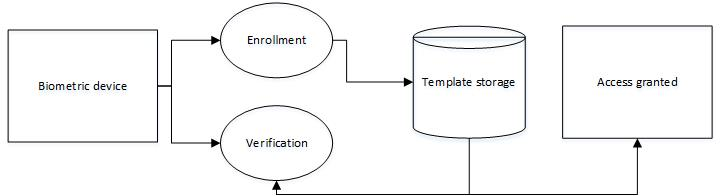
\includegraphics[width=0.8\textwidth]{Chapter1/Figs/Figure1.jpg}
\caption{ Basic authentication process model}
\label{fig:basic_authentication_process_model}
\end{figure}

The use of basic authentication systems can almost be classified as defunct, due to the fraudulent attacks becoming more commonplace. It is because of this that researchers are continuously looking for more secure forms of information protection. One of the main disadvantages of basic authentication systems is the vulnerability that occurs within storage and in transit with attackers being able to intercept sensitive authentication information at these critical points. Thus, cryptosystems were initiated. A biometric cryptosystem is an implementation technique for authenticating users by incorporating template protection (Uludag et al., 2004:948–960). One template protection scheme is known as cancelable biometrics. To classify a biometric template as cancelable, the biometric information should contain various template versions, while simultaneously being computationally irreversible. 

The concept of cryptography is predominant in steganography. Steganography is the art of surreptitiously inserting information into multimedia without changing the quality of the said multimedia (Kishor et al., 2016:1–6). This brings about the concept of combining cancelable biometrics with steganography.
The purpose of this study is to determine whether or not it is possible to improve upon biometric cancelability by using user-specific transforms, along with steganographic techniques to store biometric information.




%********************************** %Second Section  *************************************
\section{Problem Statement} %Section - 1.2


Biometrics have long been used as an accepted user authentication method and have been implemented as a security measure in many real-world systems including personal computers, mobile devices (cell phones and tablets), and physical access control (Liu \& Silverman, 2001). By encoding a person’s physical attributes the disadvantages of traditional password based security, like passwords being lost or stolen, can be overcome (Jain et al., 2016). One of the factors that hampers the acceptance of biometric authentication systems is that users have to submit private biometric data to the authentication systems and should these systems be compromised, a digital copy of their biometrics becomes available for exploitation (Rathgeb & Uhl, 2011).

The concept of Cancelable Biometrics (CB) has to do with obfuscating of biometric information that is used for biometric authentication, whether the information is in storage or in transit. This ensures that biometric information of a person cannot be reconstructed when it is observed by a third party (Shahim et al., 2016). With the use of a cancelling technique, one can assure anonymity of users within the system and prevent unauthorised usage of digitised biometric information. One of the more common methods to ensure CB is known as biometric salting (Rathgeb & Uhl, 2011). Biometric salting entails the introduction of random bits of data into the existing biometric information. Only when the random bits have been removed the original data can be obtained for use in a biometric system. This approach usually relies on a static salting algorithm which can be relatively easily reverse engineered (Shahim et al., 2016). Another approach to CB is presented by Dlamini et al. (2016), who posit that one can ensure the protection of user credentials in transit and in storage by using steganography to hide user information in images rather than in commonly used user databases. However, the approach of Dlamini et al. (2016) suffers from the same problem as that of biometric salting where the steganography process may be reverse engineered and biometric information can be reconstructed. 

To address these shortcomings, this study will include the incorporation of user biometric information as transform parameters for use in such a steganography engine as implemented by Dlamini et al. (2016). This results in a steganography algorithm that encodes a user’s biometric information in a picture based on their own unique traits rather than arbitrary algorithm parameters which may be computationally deduced. The premise is that each set of biometric information is stored in a different manner or location within an image and even when one user’s information is identified from the image, the fidelity of other users’ information remains intact because the transform parameters are unique to each user. This is opposed to when a common user database is breached and all the users’ information contained therein may be exposed. With the combination of steganography and CB this study can contribute to bridging the gap in biometric information storage and use within security systems.

To capture biometric information, Chan et al. (2015) presents the implementation of a Leap Motion Controller (LMC) to assume the role of a biometric authentication device. This is due to traditional biometric devices (such as fingerprint readers) having a high cost implication. The LMC is a relatively low cost input device that is usually used for motion control of computer systems. By harnessing the biometric information that is implicitly captured when the LMC is used, biometric authentication can be performed. 

Thus, this research proposes the development of a novel CB algorithm by employing a steganography approach for the storage and retrieval of biometric user information based on individual users’ physical traits where the information is obtained from an LMC. Investigation into the underlying hardware and software topics is warranted to determine the feasibility of these technological aspects before experimental implementation and testing can commence.


%********************************** % Third Section  *************************************
\section{Research question}  %Section - 1.3 
\label{section1.3}

Biometric cancelability can be enhanced using user-based transform parameters (obtained from an LMC) for a steganography algorithm that stores biometric information.


\section{Aim and objectives}  %Section - 1.4 
\label{section1.4}
The primary aim of this study is to develop a technique that ensures cancelability of biometrics based on hand geometry information from an LMC and steganographic storage techniques.
To achieve the primary objective, the following secondary objectives need to be met:

\begin{enumerate}[label=\roman*.]
\item Perform a literature study to discuss the use and implementation of cancelable biometrics, steganography, hand geometry authentication and the Leap Motion Controller.
\item Design and implementation of the system.
\item Evaluation of the created system using error-based metrics and iterative validation testing.
\end{enumerate}

\section{Research method}  %Section - 1.5 
\subsection{Introduction}
In this section various research paradigms that were considered for this study are will be discussed, followed by the chosen paradigm and research method for this study. The following research conducted on the paradigms is predominantly based on Oates (2006). The discussion entails an overview of the design science research method, preceded by a summary of both the interpretivistic and positivistic approaches.

\subsection{Interpretivistic paradigm}
\subsubsection{Introduction to interpretivism}
According to Oates(2006), interpretivism refers to the researcher’s ability to analyse an information system by means of comprehending the processes within its development in terms of social factors (Oates, 2006, p. 292). These social factors involve the people that created the systems and the dependencies from a social standpoint within a particular framework.
It can, therefore, be concluded that an interpretivistic approach to research is not focused on the proof or disproof of a particular theory. Instead, interpretivism has to do with the identification, researching techniques and the explanation of the social factors that contribute to holistically understanding a particular social context.
\subsubsection{Ontology \& epistemology}
The ontology of interpretivism has to do with being able to comprehend various kinds of opinions and interpretations in an attempt to combine multiple versions of the truth. The researcher should, thus, accept that his/her own personal perspectives and understanding of the particular topic will contribute to the final results that will be gained from the study.  This particular researcher should ensure that he/she possesses a non-neutral perspective in order to interpret the topic in a manner that is influence by the various social factors.
\subsubsection{Characteristics of interpretivistic approach}
Since interpretivism does not intend to prove or disprove a particular theory, it can be stated that once a social setting has been critically analysed a researcher has the ability to illustrate how social factors within the setting are associated and unified. Interpretivistic research paradigms have the following characteristics (Oates, 2006, p.292): 
\begin{enumerate}[label=\roman*.]
\item Realities that are subjective. The concept of ‘truth’ is based on perspectives and that one researcher's perception is likely to differ from another researcher’s, simply because of the construction of knowledge that takes place within each of our own minds.
\item Volatile construction to meaning based on social factors. Thus, the researcher is able to observe the world according to his/her own realities. Information may be subject to change in terms of context, time and culture.
\item Non-neutrality. Meaning that the researcher should maintain his/her right to make assumptions, to enforce his/her beliefs and to act upon these social factors in an attempt to conclude the research. This research is dependent on the researcher’s personal opinions.
\item Analysis of research subjects within their social settings. This means that the researcher attempts to comprehend people within their natural settings rather than creating an artificial setting. This is focused on trying to gain a perspective from the participant within that setting, as well as the observers and to merge the various perceptions using interpretation.
\item Data analysis using qualitative methods. Within the interpretivistic approach, the preferred data analysis technique is that of a qualitative nature. This involves the use of language, metaphors and imagery to gain multiple results and observations to be interpreted.
\item Numerous interpretations. Ultimately, the researcher does not expect to come to one specific conclusion, but rather combine all the extracted information and focus on the results that provide the most powerful evidence. This allows the researcher to interpret bulk amounts of information and finally concluding the study.
\end{enumerate}

\subsubsection{Interpretivistic critique}
Interpretivism involves studying social factors relating to specific social settings and behaviors within that setting. Therefore, interpretivism is an approach to research that involves multiple perspectives and relies on the above critique for the research to be viable rather than basing its credibility on the accuracy of data as a positivistic approach would.
\subsubsection{Interpretivistic methods}
The methods used within interpretivism are ethnography and case studies. Within these methods, it can be assumed that subjectivity is crucial to the research. 
\begin{enumerate}[label=\roman*.]
	\item Ethnography is successful if the researcher has the ability to successfully understand the activities of humans in interrelated cultures and to comprehend their social setting.
	\item Case studies have the focal point that ensures one specific ‘target’ is examined. This target can be analyzed in depth using various data gathering techniques.
\end{enumerate}

\subsubsection{Data gathering techniques and analysis}
Because interpretivistic researchers need to focus on the plausibility of a research topic, the data generation techniques are crucial in providing evidence for the conclusions that are drawn by the researcher. This evidence can be regarded as valid if they are generated using the following techniques (Oates, 2006, p.295):
\begin{enumerate}[label=\roman*.]
	\item Interviews;
	\item Observation;
	\item Document analysis; and
	\item Field notes.
\end{enumerate}

\subsection{Positivistic paradigm}
\subsubsection{Introduction to positivism}
According to Jokobsen, positivism refers to the positions within philosophy that accentuate both scientific methods, as well as, data that is empirical (Jokobsen, 2013). Within the Business Dictionary, positivism is a concept that perceives true knowledge to be that that is directly linked to scientific knowledge based on what is observed. It is then stated that empiricism is extended within positivism (Business Dictionary, 1999).
It can, therefore, be concluded that a positivistic approach to research is based on empiricism and the use of scientific methods to infer knowledge based on observations that are made once data has been gathered and analysed.
\subsubsection{Ontology \& epistemology}
The ontology of positivism is to do with the way in which the world is observed, measured and modelled by a specific researcher. This specific researcher should also ensure that he/she takes a neutral stand-point and is objective in his/her approach. 
With regards to epistemology in positivism, is can be stated that knowledge is classified into two basic forms. These forms include only knowledge that is empirical and knowledge that is logical (Oates, 2006).
It can be concluded that with a positivistic approach, the researcher should proceed in a neutral and objective manner while observing the world, using logic and empiricism as a guide for the conducted research.
\subsubsection{Characteristics of positivistic approach}
Because positivism is based on a ‘scientific approach’ to research, the researcher is expected to share a worldview with that of either positivistic researchers. Various assumptions can be made by these researchers that include common characteristics. According to Oates, these characteristics include the following (Oates, 2006, p. 286): 
\begin{enumerate}[label=\roman*.]
	\item Measuring and creation of models. The researcher is able to observe the world according to the positivistic ontology and using this view is able to create models of this perceived world according to the ‘facts’ obtained through scientific methods.
	\item The objective approach. The researcher should maintain impartiality as an observer throughout his/her research. This research must be independent of the researcher’s personal opinions.
	\item The testing of hypotheses. This refers to the use of empiricism within the testing of various theories or the refuting of these theories.
	\item Data analysis using quantitative methods. Within the positivistic approach, the preferred data analysis technique is that of a quantitative nature. This involves creation of mathematical models to logically and objectively analyse the given results and observations.
\end{enumerate}

\subsubsection{Positivism critique}
Because the positivism involves studying aspects relating to the natural world, researchers who prefer other methods are likely to impose on this technique. Positivism is a very general approach to research and it cannot always be used to generalize the ontology of things. This shows that there are not always predictable patterns and that research can evolve around various natural interpretations.
\subsubsection{Positivistic methods}
The method used within positivism is a scientific method. Within this method, it can be assumed that objectivity is crucial within our investigation, and that the world could be viewed as an orderly entity that does not operate in a random fashion (Oates, 2006, p. 283). 
With the use of the scientific method, it can be stated that various characteristics of positivism are used. Such characteristics include reducing problems, repeatability of processes and finally refuting theories. 
The scientific method runs through an iterative cycle which involves the following basic steps to ensure that knowledge is gained in the process:
\begin{enumerate}
	\item Create a theory from the perceived world;
	\item Instantiate an assumption or hypothesis;
	\item Use objectivity as a researcher to test the assumption;
	\item Analyse the results through observation;
	\item Use refutation or confirmation of the given assumption; and
	\item Deem the assumption accepted or rejected.
\end{enumerate}

In conclusion, the methods used within positivism are structured and involves a set process by stating the research assumption and then either accepting or rejecting the assumption based on objective observation and analysis.

\subsubsection{Data gathering techniques and analysis}
Various data gathering techniques may be used within positivistic research. Such techniques mainly involve experiments. However, other methods such as the sending out of surveys and questionnaires. Once these techniques have been used to gather data, the analysis of this data can then be described as quantitative. The second form of data analysis may be described as qualitative. This involves results obtained from interviews, observed data, narrations and documentation. Qualitative research focusses on data that is not always measurable and includes data such as textual data, images and audio when using techniques such as interviews etc. 
In conclusion, these data gathering techniques include methods such as interviews and surveys with the results being analysed in either a quantitative manner or a qualitative manner.
\subsection{Design science research}
\subsubsection{Overview}
A general definition for research would be an activity that aids in the detailed comprehension of a specific phenomenon (Vaishnavi \& Kuechler, 2015). In contrast to the aforementioned definition, DSR allows for creation of the phenomenon rather than the understanding thereof. Furthermore, research typically involves the comprehension of a phenomenon and allows the research to make some sort of prediction regarding the phenomenon’s outcome to contribute theory of knowledge that is deemed valid (based on knowledge and understanding gained throughout the process). Owen (1997) proposes that through action, knowledge can be generated. Critics occasionally consider this approach to lack in rigor. However, the process is far from unstructured.
What differentiates DSR from conventional design approaches is that it targets the unknown areas and explores the problems that may not have been solved yet. This is purely to challenge intellectual risk and to fill the void of missing knowledge within a research community (Vaishnavi \& Kuechler, 2015).
\subsubsection{DSR process model}
The DSR process model can be seen below in Figure ~\ref{fig:DSR_Process_Model} (Vaishnavi \& Kuechler, 2015). This precedes the descriptions of each of the phases in the next section.
\begin{figure}[ht]
\centering
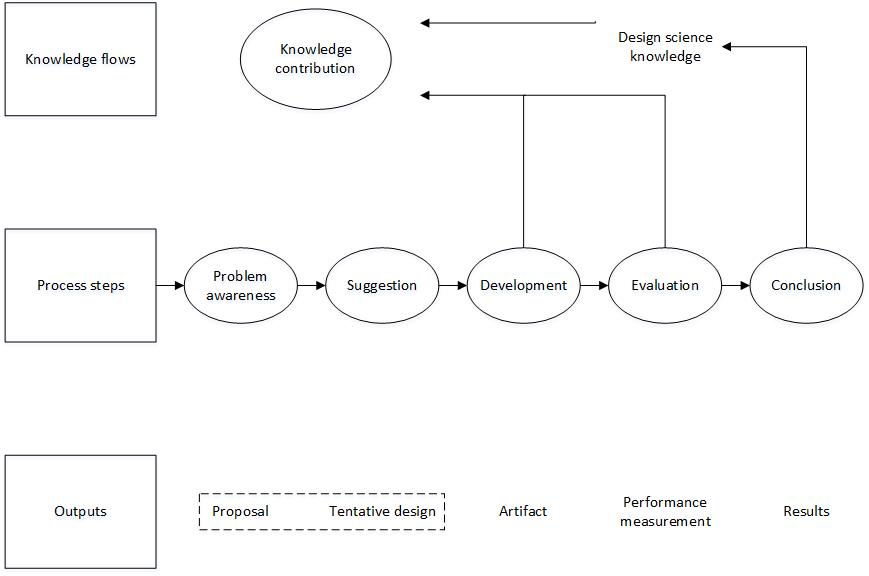
\includegraphics[width=0.8\textwidth]{Chapter1/Figs/Figure2.jpg}
\caption{DSR Process Model}
\label{fig:DSR_Process_Model}
\end{figure}

\subsubsection{Phases}
\begin{enumerate}[label=\roman*.]
	\item Awareness of the problem\\\vspace{4mm}
	To be sufficiently aware of the problem at hand it is the researcher’s responsibility to maintain constant and consistent knowledge relating to the problem from various sources (such as within allied disciplines). In this way, the researcher may come across new developments to propose improved approaches. As seen in the above figure, the output for a researcher’s awareness to a problem is ultimately a proposal.
	
	\item Suggestion \\\vspace{4mm}
	This is directly linked to the proposal as the researcher creatively displays the envisioned solution to the problem based on the awareness thereof. After having spent a considerable amount of time and effort into sufficiently comprehending the problem, if the researcher fails to produce an idea or design that suffices then the proposal will be set aside. Thus, possibly saving time that may have been spent on further research and development.
This step also cohesively ties into the positivistic approach of materialising the researcher’s curiosity relating to the phenomenon at hand.

	\item Development \\\vspace{4mm}
	The development phase merely attempts to extend upon the tentative design that was created in the suggestion phase. Implementing this phase is strongly dependent on the type of artefact to be produced. The design of the artefact may be a novelty rather than the construction thereof.
	
	\item Evaluation \\\vspace{4mm}
	Once the development of the artefact is complete, a researcher commences with evaluation thereof. This evaluation is based implicitly on criteria set out in the initial proposal. This phase is crucial to the research because any aberrations from initial anticipations must be carefully noted and thoroughly explained. It is during this phase that this positivistic approach to the problem exploration may be confirmed or acquitted. 
	
	\item Conclusion \\\vspace{4mm}
	By concluding the study, the researcher typically states whether the results sufficed the hypothesis or ‘problem exploration’ to have been accurate and justifiable by proof. These results are strengthened with knowledge gained throughout the research process and confirmed by facts observed throughout extensive studies. By concluding the study, it can be expected that a knowledge contribution be made to the specific research field.
\end{enumerate}

\subsection{Conclusion}
Upon completing the analysis of the previously discussed approaches, it was concluded that this study is positivistic in nature and should follow the DSR method. This can be motivated due to the awareness of the problem that exists within biometric authentication systems. This research intends to use that positivistic approach to verify whether or not the suggested solution will be able to enhance biometric cancelability through the development of a biometric authentication system using an LMC and steganographic techniques. Once the development of this system is complete, evaluation thereof will follow and based on the statistical data obtained, the research process can be concluded by determining whether the results justify the hypothesis.

\section{Deployment}  %Section - 1.6 
\label{section1.6}
Within Chapter 2, a literature study was conducted on related topics to the explored problem. Related research will be discussed along with the various subsections that relate to the tentative design that was created. These subsections include the concepts of biometrics, cancelability, steganography and the LMC. Furthermore, these subsections will include what each element consists of, how they work, how they suit this study and finally how they will be implemented.
In Chapter 3, the system design will be described with regards to its various elements and the chosen approach for each element will be discussed at length.
In Chapter 4, experimentation will commence by analyzing data extraction techniques, as well as testing algorithm efficiency based on extraction, processing and storing biometric information within the suggested system.
Chapter 5 will involve evaluation of the system based on implicit criteria set out within the proposal and design of the suggested model.
Finally, Chapter 6 will conclude the study by justifying the problem exploration based on results attained.

\section{Chapter summary}
\label{section1.7}
Within this chapter the basics concepts relating to this study were explained. This chapter is introductory to the purpose of the study, what the preliminary aims and objectives are and what research method will be followed. Finally, a brief over regarding the layout for the remainder of the study is given.

%!TEX root = ../thesis.tex
%*******************************************************************************
%****************************** Second Chapter *********************************
%*******************************************************************************

\chapter{Related research}

% \ifpdf
%     \graphicspath{{Chapter2/Figs/Raster/}{Chapter2/Figs/PDF/}{Chapter2/Figs/}}
% \else
%     \graphicspath{{Chapter2/Figs/Vector/}{Chapter2/Figs/}}
% \fi


\section[Introduction]{Introduction}
Complex methods are often used in an attempt to rectify basic security aspects that should be prevalent in all authentication systems but are lacking. Biometric information remains unique to each individual and it is for that reason that it should be protected, and yet many developers neglect the importance of securing biometrics effectively. Due to this negligence, this research aims to present a novel approach for authentication systems to protect biometric information using a combination of transformation techniques and steganography encryption methods subsequent to the biometric information being captured by a leap motion controller. 

Within this chapter, an overview of the related topics will be given, followed by their current uses, implementations and relevance to this particular study. These topics include biometrics, cancelability, steganography and the use of a Leap Motion Controller peripheral device. Finally, the chapter will be concluded by coalescing the various techniques to provide theoretical proof of concept for the proposed authentication system.


\section[Biometrics]{Biometrics}
Biometrics have long been used as an accepted user authentication method and have been implemented as a security measure in many real-world systems including personal computers, mobile devices (cell phones and tablets), and also physical access control systems \citep{Shahim2016}.

Biometrics are the digitalisation and analysis of a person’s innate physical or biological characteristics and the use thereof to distinguish between persons that are to be afforded access to specific systems, information or physical areas \citep{Rathgeb2011}. By encoding a person’s physical attributes the disadvantages of traditional password based security, like passwords being lost or stolen, can be overcome \citep{Verma2016}. One of the factors that hampers the acceptance of biometric authentication systems is that the cost of the development and implementation has traditionally been high due to factors such as biometric hardware, computational processing power, infrastructure integration, user training, and research and testing (Verma \& Sinha, 2016). Furthermore, biometric systems present a unique challenge in terms of user privacy due to the personal nature of the biometric information that is stored in and used by the system \citep{Paul2012}.

The cost factor is one that decreases as continued development in the related hardware takes place. Alongside this development of dedicated biometric hardware there is an influx of new augmented computer interaction possibilities (i.e., new and non-traditional ways to control computers), a wide range of technological facets such as voice-, imaging- and movement control are receiving a lot of attention \citep{Paul2012, Verma2016}. Voice-control consists of verifying who the speaker is with the use of voice biometrics. This type of biometric has shown vast improvement recently and is often used to prove that low error-rates combined with high accuracy is achievable with its use. Image-control typically refers to facial recognition implementations, retina scanners and/or eye-tracking software that implement infrared imaging. In order to facilitate these interactions, the hardware is implicitly working with information that can be harnessed for biometric authentication. Hardware peripherals (like the leap motion controller (LMC)) that extend the basic functionality of computers to include support for voice and imaging facets are becoming more commonplace \citep{Rathgeb2011}. These peripherals are even used in biometrics research. For instance, \cite{Chan2015}, use an LMC for hand scanning and biometric authentication whereby a user would be able to gain access to a system, physical area or information by having their hand geometry scanned and analysed. They also posit the use of an LMC in multifactor authentication systems in combination with traditional passwords and PIN approaches. 
Typically, this type of biometric authentication process follows the protocol of matching prior biometric templates (i.e. digitally formatted biometric features) that are stored within a database to the biometrics that are presented to the system during the biometric scanning process. 

This study proposes a system that expands on the existing techniques for biometric authentication with an LMC. This expansion uses techniques from steganography to store binary representations of the biometrics within an image as a biometric template alternative. The system does not merely store the raw biometric data within the image, but rather applies transform parameters to it. Only once the transform parameters have been added to the original biometrics are they stored/matched to authenticate and authorise the user. This ensures that each users’ biometric information is neither compromised, nor exposed. 

Cancelable biometrics refers to protecting the biometric information from third party scrutiny by obfuscating this information. This addresses the challenge of privacy of biometric information as mentioned above and is further discussed in the next section.


\section[Cancelability]{Cancelability}
With the use of authentication systems becoming more prevalent, a primary concern becomes real-time processing of transmitted information as to verify a user’s identity. The authentication process itself within traditional systems has evolved and often resorts to biometric information rather than passwords, tokens and/or secret keys \citep{Verma2016}. This is primarily due to the inability of these traditional schemes to differentiate between an authentic user and an impostor. By authenticating users using biometric information the privacy of biometric data becomes important. Should attackers manage to gain access to the recognition system and its underlying data, the user-specific biometric information becomes readily available for identity theft. 
A possible solution would be to use multifactor biometric authentication with two or more biometric traits being employed. However, by adding more biometric features it will only add to the possible losses (should the system be compromised). Within the information security industry, one of the long acclaimed benefits of using biometric authentication has been that with post-enrolment biometric templates, user-specific biometric information (matching the stored template) could not be reconstructed. The benefit was refuted and once biometric templates become compromised, the biometric template is rendered useless \citep{Rathgeb2011}. This is because unlike passwords, biometric templates cannot simply be re-assigned due to their personal unique nature. Considering the susceptibility of such biometric authentication systems an approach to enhance the robustness can be used that is known as cancelable biometrics (CB). This approach improves upon standard encryption algorithms that expose biometric templates during the authentication attempt by not supporting the comparison of templates within the encrypted domain \citep{Rathgeb2011}. Simply put, the encrypted domain referred to by CB ensures that data will remain secure in transit and in storage. Furthermore, CB allows for re-issuing and/or regenerating biometric information with a unique and independent identity. The process of transforming or repeatedly distorting the biometric feature using transform parameters that are predetermined rather than using the original biometric achieves this \citep{Shahim2016}. As to meet some of the major requirements regarding biometric information protection, biometric cryptosystems (BCS) and CB are designed so that biometric features are \citep{Rathgeb2011, Verma2016}:

\begin{enumerate}[label=\roman*.]
	\item Diverse – Unable to be applied in multiple applications;
	\item Reusable – Reused/replaced in the event of compromise; and
	\item Irreversible – Computationally challenging to reconstruct the original biometric template, but simultaneously rudimentary to generate the protected biometric template.
\end{enumerate}

Various approaches may be adopted when considering an implementation schema for biometric systems. However, one must consider the alternatives to an approach as to ensure that the chosen method is feasible. Thus, both BCS and CB are presented in order to gain an objective understanding. 
BCSs are systems designed so that digital keys can be directly bound to a particular biometric \citep{Rathgeb2011}. One BCS approach is relevant to this particular study, namely biohashing which implements biometric key-generation. However, \cite{Rathgeb2011} state that an implementation should not exist that directly generates keys from biometric templates. They elaborate that biometric features cannot provide sufficient information to reliably obtain lengthy and renewable keys without relying on helper data. Helper data is public information that is used within the key generation/retrieval process in a BCS \citep{Rathgeb2011}.  This is useful to the study because helper data can be used to transform and obscure biometric information. Another approach to BCS is a biometric key-bind cryptosystem. This involves a secret key that relates to a biometric model by using helper data. To successfully implement this approach, facts regarding both the biometric model and the secret key may not be disclosed \citep{Eng2016}. According to \cite{Paul2014} and \cite{Rathgeb2011}, implementation of key-binding cryptosystems can occur through a fuzzy commitment and a fuzzy vault. The concept of fuzzy incorporates the generation of helper data extracted from biometric features using a secrecy key. The above-mentioned helper data, combined with the secrecy key are then both encrypted and stored in the database. In order to authenticate a user, the helper data then uses the model and biometric features to rebuild the key \citep{Eng2016}. A structural representation of this method can be seen below in Figure \ref{fig:System structure for biometric authentication}.

% Figure - System structure for biometric authentication figure

\begin{figure}[htbp!] 
\centering    
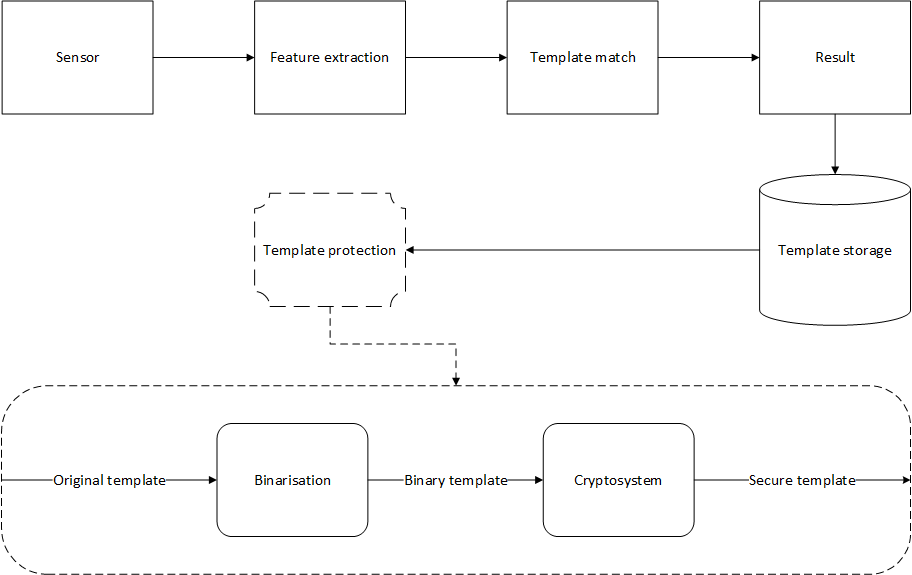
\includegraphics[width=1.0\textwidth]{Chapter2/Figs/Figure2-1.png}
\caption[System structure for biometric authentication]{System structure for biometric authentication}
\label{fig:System structure for biometric authentication}
\end{figure}

Initially, the sensor extracts the specific biometric features from the user (post-enrolment). Once the features have been extracted from the users, the current information within the system is then matched to that of the template that is stored within the database. However, during enrolment of the user in a BCS, the template that was created for each user undergoes a protection process that transforms the template into a secure template. The above-mentioned template protection process includes the binarisation of the extracted biometric features. Once the binary template is created, the template is then further processed by the cryptosystem to ultimately generate the secure template. This means that each time the user attempts to be authenticated, the extracted features use the helper data to rebuild the key and match the generated template to the secure template. Finally, if the templates match then the result will be positive and the user will gain access. 
Having considered a BCS, one needs to weigh up the options regarding the possible approaches to cancelability and implementations thereof. Cancelability, too, has the sole purpose of ensuring computational challenges when attempting to retrieve/recover the original biometric data by a third party (Rathgeb \& Uhl, 2011:1–25). The focal point regarding cancelability remains that biometric characteristics should remain innately robust so that even when transform parameters are applied the biometric features do not lose value/individuality. Along with individuality, by transforming biometrics one should ensure tolerance to intra-class variance so that the False Rejection Rate is not too high. Another important feature that cancelability has to offer is unlinkability \citep{Rathgeb2011}. This ensures that multiple transformed templates do not reveal any information relating to the original biometrics. In the unlikely event of data compromise, the transform parameters are simply altered which simultaneously implies biometric template updates. 
With regards to transforms within a CB implementation, two categories are forthcoming, namely \citep{Jain2016}:
  

\begin{enumerate}[label=\roman*.]
	\item Non-invertible transforms; and
	\item Biometric salting.
\end{enumerate}

The above-mentioned approaches differ in performance, accuracy and security. Depending on the system that is to be implemented, a weighted feasibility analysis should be conducted on those particular factors in order to select the most suitable approach. These approaches are briefly discussed below.

	\subsection{Non-invertible transforms}
	This approach involves the use of a non-invertible function that is applied to the biometric template. By applying this function, stored templates can be updated when transform parameters are modified \citep{Piciucco2016,Rathgeb2011}. Therefore, security is increased due to the inability to reconstruct the biometric data even though transforms may have been compromised. With this advantage comes an equal and opposite disadvantage. A loss of accuracy and a performance decrease is the disadvantageous result thereof. This is due to transformed biometric templates becoming laborious in comparison processing, which ultimately provides fewer biometric results to process during matching (thus, influencing the accuracy thereof).
	
	\subsection{Biometric salting}
	Biometric salting commonly involves biometric template transforms that are preferred invertible as opposed to the non-invertible approach (mentioned above). The term “salting” refers to the act of merging specific data (such as passwords) with unique random values (“salt”) in order to make all of the original data distinct \citep{SyedAhmad2012}. In this particular context, this technique may be applicable when a 4-digit PIN is used as the salt to be combined with the hand geometry vector prior to hashing the combination of data. This means that regardless of what biometric feature vector is chosen, the biometric template extraction cannot be reconstructed to the original biometric template \citep{Paul2014,Rathgeb2011}. This commands that transform parameters have to remain private. Variations of the approach may appear if user-specific transforms are applied. However, this demands that each authentication attempt requires transform parameters which may result in discrepancies if attackers successfully attain transform parameters. Ultimately, a decrease in performance is likely if the system implementation does not contain efficient biometric algorithms with high accuracy regarding private transform parameters. In contrast to non-invertible transforms, this approach maintains high recognition performance, however, the latter excels in terms of security \citep{Radha2011, Rathgeb2011}.



According to \cite{Rathgeb2011}, even though it is more common to adopt non-invertible approaches to system implementation schemes, biometric salting proves superior. Not only does biometric salting increase performance, but in user-specific transform applications by incorporating two-factor authentication one can improve both security and accuracy.

By taking a closer look at the general structure of using cancelable biometric we can see that during the enrolment phase, the features are extracted, transformed and then stored \citep{Patel2015}. This structure can be seen in the figure ~\ref{fig:Cancelable biometric system structure} below.

% Figure - Cancelable biometric system structure

\begin{figure}[htbp!] 
\centering    
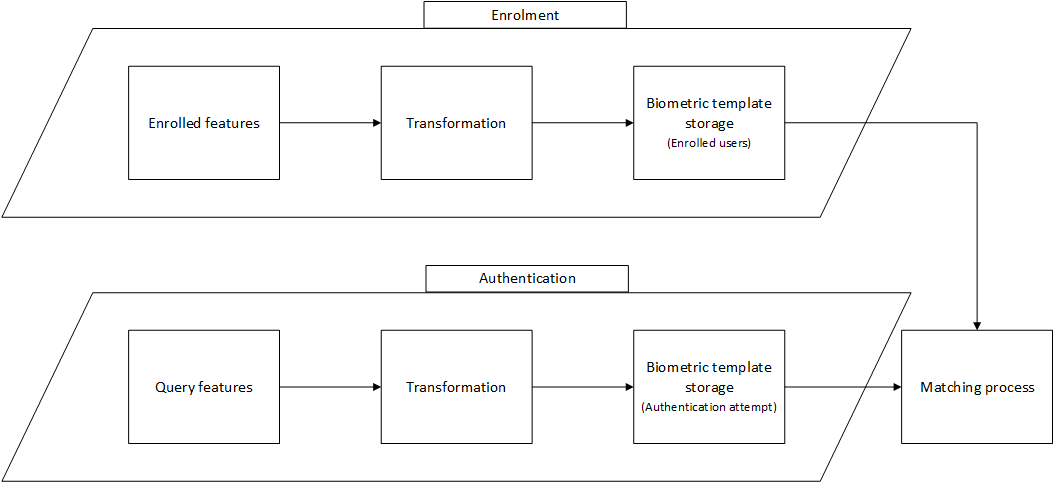
\includegraphics[width=1.0\textwidth]{Chapter2/Figs/Figure2-2.png}
\caption[Cancelable biometric system structure]{Cancelable biometric system structure}
\label{fig:Cancelable biometric system structure}
\end{figure}

The CB system structure is closely related to that of the BCS structure, however, the fundamental differences between the two are noticeable when attention is given to the timing of template protection. To argue these differences notice that in Figure ~\ref{fig:System structure for biometric authentication} the template protection occurs post-storage, whereas, in Figure ~\ref{fig:Cancelable biometric system structure} the template protection occurs after the feature extraction and prior to the storage during the transformation phase. Template protection is crucial within an authentication system with regards to attacks conducted upon the system. These template attacks will be further discussed below.

    \subsection{ Biometric template attacks}
    
    Conventional biometric systems have been subjected to numerous infiltration attacks that technologies such as BCS and CB appear to have been able to avert \citep{Rathgeb2011}. However, these techniques are known to have vulnerabilities. By analysing the structure of a generic biometric system, we are able to determine which particular processing points are vulnerable to attacks. The Figure ~\ref{fig:Vulnerability points for biometric system attacks} below illustrates some of the above-mentioned vulnerabilities \citep{Patel2015}.
    
    % Figure - Vulnerability points for biometric system attacks
    
    \begin{figure}[htbp!] 
    \centering    
    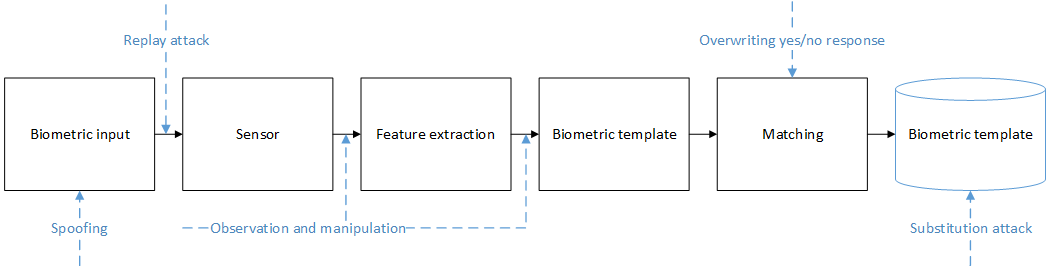
\includegraphics[width=1.0\textwidth]{Chapter2/Figs/Figure2-3.png}
    \caption[Vulnerability points for biometric system attacks]{Vulnerability points for biometric system attacks}
    \label{fig:Vulnerability points for biometric system attacks}
    \end{figure}
    
    Research shows that there are numerous vulnerable points to attack a generic biometric system \citep{Ratha2001}. However, an overview of the five points of attack mentioned above in Figure ~\ref{fig:Vulnerability points for biometric system attacks} is presented as follows \citep{Karimovich2016, Patel2015, Ratha2001, Rathgeb2011}:
    
    \begin{enumerate}[label=\roman*.]
    
        \item Spoofing – This type of attack is implemented through the presentation of a   biometric to the biometric input (sensor). An example of this type of attack includes presenting a fake finger to the sensor and so forth.
        \item Replay attack – The use of this form of attack generally involves the resubmission of biometric data that is digitally stored which ultimately bypasses the biometric input device.
        \item Observation and manipulation – There are two entry points combined for this particular attack. The first entry point would attempt to attack the feature extractor with a Trojan horse in order to produce multiple feature sets that are specified by the attacker. The second entry point attempts to corrupt the manner in which the features are represented (with the assumption that the attacker is aware of the layout produced during feature extraction). Typically, the transition from extraction to matching is seamless, but should this process occur using the internet, then this attack becomes a real concern.
        \item Overwriting yes/no response – The process of gaining access to the internal decision module and overwriting the final authentication decision. Simply put, this is a false acceptance attack.
        \item Substitution – Also referred to as a blended substitution attack. During this attack, the stored template is amalgamated with that of the attacker and used to authenticate.

    \end{enumerate}
    
    With the above-mentioned potential attacks in mind, the affected techniques and their potential attack formats should be classified. The attacks in correlation to BCS and CB can be seen in Table ~\ref{table:Technique vulnerabilities} below.
    
    % Table - Technique vulnerabilities
    
    \begin{table}[h]
    \caption{Technique vulnerabilities}
    \centering
     \begin{tabular}{|p{0.45\textwidth} | p{0.45\textwidth}|} 
     \hline
    	\textbf{Potential attacks} & \textbf{Affected techniques(s)} \\ [1ex] 
     \hline\hline 
     Spoofing & BCS and CB  \\[1ex]
     \hline 
     Replay attack & BCS and CB \\[1ex]
     \hline
     Observation and manipulation & BCS and CB\\[1ex]
     \hline           
     Overwriting yes/no response & CB\\[1ex]
     \hline
     \end{tabular}
     \label{table:Technique vulnerabilities}
    \end{table}
    
    
    By considering both techniques and how each technique is vulnerable to diverse forms of attack, it is important to consider how to protect user biometrics against reconstruction. While analysis of template protection schemes are often rigorously analysed, the methods used for biometric feature transformation have not been the focal point of most approaches \citep{Nagar2009}. The protection of the user information throughout the use of information remains crucial to the ongoing research of this particular system. 
    
    In an attempt to meet the requirement of non-invertible transforms, the use of a one-way hash algorithm could be applied to the transformed parameters as a final step prior to the matching process. The chosen algorithm standard will now be further discussed.

    \subsection{ Secure Hashing Algorithm}
    
    Cryptographic hash functions are designed to block malicious attempts of data modification \citep{Pfleeger2015}. The National Institute of Standards and Technology (NIST) is responsible for publishing the Secure Hash Standard (SHS) and is implemented in an attempt to overcome various attacks. 
    
    The term Secure Hashing Algorithm (SHA) is a term used to describe the above-mentioned standard that can be further divided into four specific algorithms, namely SHA-0, -1, -2 and -3. The purpose of such an algorithm is to compute electronic data in a manner that produces a condensed representation of a message \citep{Foti2015}. The aforementioned representation is commonly known as a “message digest” or “hash.” The length of this message digest remains constant, regardless of the length of the original electronic input data. The algorithmic process that is followed (by all four algorithms as seen below) is one that is both iterative, as well as, unidirectional. By processing electronic data in such a manner, the algorithm ensures the integrity thereof. This is because in the event that the original data should be altered in the slightest, the resulting message digest will be completely contrasting to the message digest of the original data. 
    
    To liken the various versions of the SHA algorithms, a further analysis of each of the algorithms in terms of maximum input message size, block size, number of rounds executed and message digest size is presented. The SHA comparisons can be seen in Table ~\ref{table: SHA comparisons}
    
    % Table - SHA comparisons
    
    \begin{table}[h]
    \caption{SHA comparisons}
    \centering
     \begin{tabular}{|p{0.18\textwidth} | p{0.18\textwidth}| p{0.18\textwidth}| p{0.18\textwidth}| p{0.18\textwidth}|} 
     \hline
    	\textbf{Algorithm} & \textbf{Maximum input message size (bits)} & \textbf{Block size(bits)} & \textbf{No. of rounds executed} & \textbf{Message digest size (bits)} \\ [1ex] 
     \hline\hline
     SHA-1 & \[ <2^{64}\] & 512 & 80 & 160 \\[1ex]
     \hline
     SHA-2-224 & \[ <2^{64}\] & 512 & 64 & 224 \\[1ex]
     \hline
     SHA-2-256 & \[ <2^{64}\] & 512 & 64 & 256 \\[1ex]
     \hline           
     SHA-2-384 & \[ <2^{128}\] & 1024 & 80 & 384 \\[1ex]
     \hline      
     SHA-2-512 & \[ <2^{128}\] & 1024 & 80 & 512 \\[1ex]
     \hline
     SHA-3-256 & \centering{Unlimited} & 1088 & 24 & 256 \\[1ex] 
     \hline
     SHA-3-512 & \centering{Unlimited} & 5761 & 24 & 512 \\[1ex]
     \hline
     \end{tabular}
     \label{table: SHA comparisons}
    \end{table}
    %TODO: Ref footnote
    It is important to note that prior to this study, the SHA-1 algorithm was broken by Google. A hash function is considered broken when two files happen to produce the same hash value (collision). The way in which this particular attack on SHA-1 occurred was through the use of a chosen-prefix attack. Google managed to use a precise piece of data that was injected into of the files. This caused the files to numerically align during the calculation process \citep{Stevens2017}.
    
    It was decided that SHA-2-256 would be further studied and implemented upon learning of the aforementioned collision and upon analysis of this table. Supplementary reasons for this choice include:
    
        \begin{enumerate}[label=\roman*.]
            
            \item SHA-2 has yet to be broken (unlike its predecessors);
            \item SHA-2-256 has a lower block size than those that follow; \item SHA-2-256 executes 64 rounds of hashing rather than 80; and
            \item A message digest of 256 bits is produced.

        \end{enumerate}
    
    Regardless of which SHA algorithm is chosen, the core functionality remains similar in the generation of unique hash values for any input that is fed into the algorithm. Each algorithm can be further divided into two phases, namely pre-processing and hash computations. To better explain the process followed within each of the two phases, see the Table ~\ref{table: SHA phases} below \citep{Foti2015}.
    
    % Table - SHA phases
    
    \begin{table}[h]
        \caption{SHA phases}
        \begin{tabular}{|p{0.45\textwidth} | p{0.45\textwidth}|}
          \hline
         \textbf{Pre-processing} & \textbf{Hash computation} \\
         \hline\hline
            \begin{enumerate}
                \item Padding a message;
                \item Parsing the padded message into \textit{m}-blocks; and
                \item Setting initialisation values for hash computation.
            \end{enumerate}
             & 
             \begin{enumerate}
                 \item Generates a message schedule from the padded message (along with functions, constants and word operations to iteratively generate a series of hash values; and
                 \item Uses the final hash value to determine the message digest.
             \end{enumerate} \\
             \hline
        \end{tabular}
        \label{table: SHA phases}
    \end{table}
    
    The entire SHA-2-256 algorithm can be summarized using the following equations.
    
    % SHA Equations 
    
    \begin{enumerate}
        
        \item \[W_t=\begin{cases}
                        M^{(i)}_t &, 0 \leq t \leq 15\\
                        ROTL[(W_{t-2} + W_{t-7} + \sigma(W_{t-15}) + W_{t-16}  &, 16 \leq t \leq 63
                        \end{cases}\]
 
        
        \item Initialise the 8 working variables, a, b, c, d, e, f, g and h, containing hash values for (i-1): 
            \begin{gather*}     
                a = H^{(i-1)}_0, b = H^{(i-1)}_1, c = H^{(i-1)}_2, d = H^{(i-1)}_3, e = H^{(i-1)}_4, f = H^{(i-1)}_5, g = H^{(i-1)}_6, h = H^{(i-1)}_7 
            \end{gather*}
        \item For t = 0 to 63:
            \begin{gather*}
                T_1 = h + \sum_{1}^{(256)}(e) + Ch(e,f,g) + K^{(256)}_t \\
                T_2 = \sum_{0}^{(256)}(a) + Maj(a,b,c) \\
                h = g, g = f, f = e, e = d + T_1, d = c, c = b, b = a \\
                a = T_1 + T_2 \\
            \end{gather*}
        
        \item Compute the intermediate hash values:
            \begin{gather*}
                H^{(i)}_0 = a + H^{(i-1)}_0, H^{(i)}_1 = b + H^{(i-1)}_1, H^{(i)}_2 = c + H^{(i-1)}_2, H^{(i)}_3 = d + H^{(i-1)}_3, \\ 
                H^{(i)}_4 = e + H^{(i-1)}_4, H^{(i)}_5 = f + H^{(i-1)}_5, H^{(i)}_6 = g + H^{(i-1)}_6, H^{(i)}_7 = h + H^{(i-1)}_7
            \end{gather*}
    \end{enumerate}
    
    To better explain the algorithm functionality, a use-case for this study will be hashed using the SHA-2-256 algorithm in the form of a digital representation of hand measurements. These measurements can be summarised in text format as 11,12,13,14,15. Each number represents a transformed value for each of the five fingers.
    
    
        
        \subsubsection{ Pre-processing}
        First, each letter will be converted to binary. A one is added to the end to mark the end of the phrase. Next, get the phrase size. In this case, 112-bits. Eight bits per letter makes it 112-bits and the rest get padded with zeros to get the block to the correct size. 
        
        \begin{enumerate}[label=\roman*.]
            
            \item 11,12,13,14,15 = 00110001 00110001 00101100 00110001 00110010 00101100 00110001 00110011 00101100 00110001 00110100 00101100 00110001 00110101 (112-bits);
            
            \item Add 1 to mark the end of the phrase;
            
            \item Pad the message with zeros (375-bits);
            
            \item Get the size of the phrase (11,12,13,14,15) = 24-bits.
            
        \end{enumerate}
        
        Upon completion of the four steps required for pre-processing, a block of 512 bits is formed and is presented in the Table ~\ref{table:Pre-processing bit block example} below:
        \begin{table}[h]
            
            \caption{Pre-processing bit block example}
            \label{table:Pre-processing bit block example}
            \begin{center}
            \begin{tabular}{|c|}
             \hline     
             0011000100110001001011000011000100110010001011000011000100110011 \\
             001011000011000100110100001011000011000100110101\underline{1}000000000000000 \\
             0000000000000000000000000000000000000000000000000000000000000000 \\
             0000000000000000000000000000000000000000000000000000000000000000 \\
             0000000000000000000000000000000000000000000000000000000000000000 \\
             0000000000000000000000000000000000000000000000000000000000000000 \\
             0000000000000000000000000000000000000000000000000000000000000000 \\
             000000000000000000000000000000000000000000\textbf{1100010011000100110010} \\
             \hline
            \end{tabular}
            \end{center}
            
        \end{table}
        
        The message scheduler needs 64 words to be created from the block, but with each word being only 32-bits long, we only have enough for 16 words. 
        
        \begin{table}[h]
            \caption{Pre-processing bit block divided into 32 bit words}
            \centering
            \label{table:Pre-processing bit block divided into 32 bit words}
            
            \begin{tabular}{|c|}
            \hline  

            
              1. 00110001001100010010110000110001 \\
             
              2. 00110010001011000011000100110011 \\
             
              3. 00101100001100010011010000101100 \\
             
              4. 00110001001101011000000000000000 \\
             
              5. 00000000000000000000000000000000 \\
             
              6. 00000000000000000000000000000000 \\
             
              7. 00000000000000000000000000000000 \\
             
              8. 00000000000000000000000000000000 \\
             
              9. 00000000000000000000000000000000 \\
             
              10. 00000000000000000000000000000000 \\
             
              11. 00000000000000000000000000000000 \\
             
              12. 00000000000000000000000000000000 \\
             
              13. 00000000000000000000000000000000 \\
             
              14. 00000000000000000000000000000000 \\
             
              15. 00000000000000000000000000000000 \\
             
              16. 00000000001100010011000100110010 \\
             
            \hline
            \end{tabular}
        \end{table}
        
        
        This algorithm formally describes how to create the other words. 
        % Equation for algorithm
        \begin{gather}
             \textbf{ROTL} [(W_{t-2}) + W_{t-7} + \sigma_0(W_{t-15}) + W_{t-16}]
        \end{gather}
        
        
        To get the 17th word, get the word 15 places back, in this case the second word, make 2 copies of it and right-rotate one of them by 7 places. This means each number moves one place to the right, 7 times, and when a number falls off the edge, it comes back on the other side. Right rotate the other by 18 places. Then right shift the last copy by 3. Right shift means that when a number falls off the edge, they are replaced with zeros on the other side. Do the same for the word 2 places back, 15th word, except right rotate by 17 and 19 places. Then right shift by 10. Add it to the word 16 places back, the 1st word and the words 7 places back, 10th word. Add all of these together and we get the 17th word. Proceed like this until we get 64 words. 
        
        \subsubsection{ Hash computation}
        
        The last part of the algorithm (step 3) uses the eight initial hash values and the 64 constant values. By converting between base 2 and base 16 is ultimately what produces the complex final signature. Table ~\ref{table:Initial hashes and K-Constants} illustrates the aforementioned conversions with the final signature.
        
        
        % Table - Initial hashes and K-Constants
            
        \begin{table}[h]
        \caption{Initial hashes and K-Constants}
        \begin{tabular}{{|p{0.2\textwidth} | p{0.80\textwidth}|}}
          \hline
         \textbf{Initial hashes} & \textbf{K-Constants} \\
         \hline\hline
            \rule{0pt}{4ex}
                H(0) = a09e667 & 428a2f98 71374491 b5c0fbcf e9b5dba5 3956c25b 59f111f1 923f82a4 \\
                H(1) = b67ae85 & ab1c5ed5 d807aa98 12835b01 243185be 550c7dc3 72be5d74 80deb1fe \\
                H(2) = 3c6ef372 & 9bdc06a7 c19bf174 e49b69c1 efbe4786 0fc19dc6 240ca1cc 2de92c6f \\
                H(3) = a54ff53a & 4a7484aa 5cb0a9dc 76f988da 983e5152 a831c66d b00327c8 bf597fc7 \\
                H(4) = 510e527f & c6e00bf3 d5a79147 06ca6351 14292967 27b70a85 2e1b2138 4d2c6dfc \\
                H(5) = 9b05688c & 53380d13 650a7354 766a0abb 81c2c92e 92722c85 a2bfe8a1 a81a664b \\
                H(6) = 1f83d9ab & c24b8b70 c76c51a3 d192e819 d6990624 f40e3585 106aa070 19a4c116 \\
                H(7) = 5be0cd19 & 1e376c08 2748774c 34b0bcb5 391c0cb3 4ed8aa4a 5b9cca4f 682e6ff3 \\
                                & 748f82ee 78a5636f 84c87814 8cc70208 90befffa a4506ceb bef9a3f7 \\
                                & c67178f2 \\  
        \hline
        \end{tabular}
        \label{table:Initial hashes and K-Constants}
        \end{table}
       
        To get T1, us the value of \textit{e} and create three new words by right rotating by 6. 11 and 25. Then do an XOR on these values. Then run the Choose function of e, f and g. Get the first K constant, the value of h and the 1st word from the message scheduler and calculate the AND of all of these. 
        
        To get T2, run the Majority function over a, b and c. Then create 3 new words by Right Rotating a by 2, 13 and 22. Then get the XOR of all of these and swap and modify the values as seen in the function.  
        
        This process is then repeated 64 times. 
        
        Lastly, AND the values that we had initially for the hashes to the corresponding final values and concatenate them all together to produce the final message digest.
        
        % Equation 
        
        \begin{gather}
            H^{(N)}_0 || H^{(N)}_1 ||H^{(N)}_2 || H^{(N)}_3 || H^{(N)}_4 || H^{(N)}_5 || H^{(N)}_6 || H^{(N)}_7 
        \end{gather} 
        
        An example of a message digest can be seen when hand geometry measurements that have undergone transforms produce an initial output (prior to hashing) of: 

        \begin{center}
            \textbf{\textit{11,12,13,14,15}}
        \end{center}
        
        By using the SHA-1 hash algorithm, we see a message digest (160 bits) of:
        
        \begin{center}
            \textbf{\textit{b4bf77f04af433a2ed748a44760f043acec04e35}}
        \end{center}
        
        With the same input string, using SHA-2-256 we see a message digest (256 bits) of:
        
        \begin{center}
            \textbf{\textit{2c72ea316fc05ec89ede357ebe416fb80214396889462c07546978c18445310d}}
        \end{center}
        
    

Ultimately, this message digest would then be stored rather than the plaintext of the original data.

To conclude this subsection, the aim is to combine the key-binding capabilities of a BCS, the secure hashing algorithm and the biometric salting of CB. Once the user-specific biometric information has been transformed and is secure, it is ready for storage. In order to store this sensitive biometric information, rather than using a conventional database (due to its vulnerabilities, i.e. username/password exploits) a technique known as steganography was utilized and is described in the next section. 


\section[Steganography]{Steganography}
According to \cite{Kishor2016}, secret information is hidden using a type of communication, known as steganography. This is done through the use of multimedia files in conjunction with secret keys to embed information within these multimedia files. Steganography came about when it was realised that cryptography itself was incapable to securely transmit various forms of information across the internet \citep{Jain2016}. The word steganography can be translated from Greek into “covered writing” \citep{Pandit2016}. When hiding sensitive information, the information in question is typically concealed using an alternative format to that of its original. This is done through regeneration of data using multimedia formats. Some of these formats include text, image, audio and even video. For the purposes of this particular study, focus will be maintained upon image steganography and the shrouding of sensitive biometric information by means of bit encryption within the cover object (image). While cryptography disguises only the meaning of a message using code, steganography aims to hide the entire message from possible attackers \citep{Kishor2016, Pradhan2016}.

The conventional flow of image steganography (as seen in Figure ~\ref{fig:Conventional image steganography flow}) follows a combination of encryption and decryption (just as cryptography does), but aims to use a confidential communication channel while secretly storing data and protecting the alteration of that data. An application that also makes this technique crucial to this particular study is the use of steganography as a conventional database alternative \citep{Pandit2016}.

% Figure - Conventional image steganography flow

  
\begin{figure}[htbp!] 
\centering    
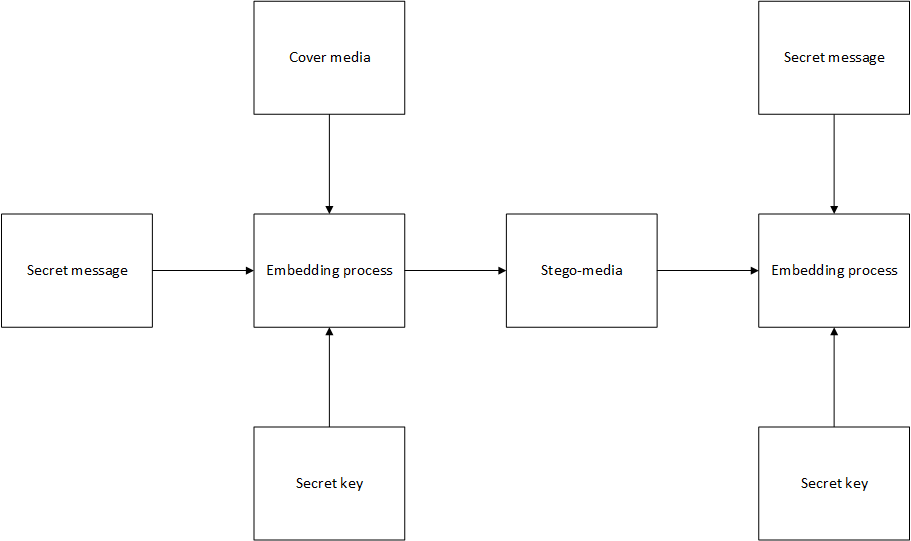
\includegraphics[width=1.0\textwidth]{Chapter2/Figs/Figure2-4.png}
\caption[Conventional image steganography flow]{Conventional image steganography flow}
\label{fig:Conventional image steganography flow}
\end{figure}

In image steganography, both the encryption process and the decryption process involve the use of a cover image and a stego-image. In short, the difference between the two is merely that the stego-image contains the sensitive information, while the cover image can be seen as an empty data storage location for the sensitive information. In Figure ~\ref{fig:Conventional image steganography flow}, the steganography process requires sensitive information that is to be stored within the cover media (in this case, the image). This sensitive information is embedded into the image with the use of a secret key and a cover image to hide the information in. With the embedded information, the image is then referred to as the “stego-image.” The sensitive information can then only be extracted if the secret key is known.

Steganography can be implemented in various ways. However, the two major techniques that will be discussed regarding image steganography involve the following \citep{Pradhan2016, Paul2012}:

\begin{enumerate}[label=\roman*.]
	\item Spatial domain technique; and 
	\item Transform domain technique.
\end{enumerate}

The main difference between the two techniques is that when implementing a spatial domain steganography, the pixels within the image are directly manipulated. This is juxtaposed to the transform domain steganography that uses distinct transformations to allow image transformation in the transform domain and then only is the sensitive information stored with the image \citep{Pradhan2016, Roy2016}.

Literature broadens the scope of steganography even more in stating that spatial and transform domain techniques branch out into subcategories of implementation \citep{Radha2011, SyedAhmad2012, Verma2016}. A few examples of these methods can be seen in the Table ~\ref{table: Steganography methods}.

\begin{table}[h]
\caption{Steganography methods}
\centering
 \begin{tabular}{|p{0.45\textwidth} | p{0.45\textwidth}|} 
 \hline
	\textbf{Spatial Domain} & \textbf{Transform Domain} \\ [1ex] 
 \hline\hline 
 Least Significant Bit substitution & Discrete Cosine Transform  \\[1ex]
 \hline 
 Pixel Value Differencing & Discrete Wavelet Transform  \\[1ex]
 \hline
 Random pixel selection & Discrete Fourier Transform  \\ [1ex] 
 \hline
 \end{tabular}
 \label{table: Steganography methods}
\end{table}


The purpose of modern steganography is to allow the host image protection so that the image itself, as well as the sensitive data it holds may not be recovered from the stego-image. By achieving this, the technique implemented is classified as irreversible steganography. The aforementioned objective is typically partnered with the ability to conceal sensitive information in a natural image in such a way that distortion of that image is minimal.

It is important to maintain that this particular study focusses on cancelable biometrics being stored using steganography techniques. This implies that the image may be distorted because even if an attacker manages to access the stego-image, he/she should not know what type of information is being stored, nor how to recover to biometrics after the transforms. 

According to \cite{Jain2016} and \cite{Pradhan2016}, steganography techniques are evaluated using various criteria. However, evaluation criteria that is relevant to this particular study are the following:

\begin{enumerate}[label=\roman*.]
	
	\item Hiding capacity – This is the maximum amount of data that can be stored within an image with reference to bits per pixel (bpp). Comparatively speaking, a larger hiding capacity means the steganography technique is better.
	
	\item Security Analysis – The technique should be able to withstand attacks to the image that include any attempt to alter the image.
	
	\item Robustness – By being robust against attempts to attack the image statistically, as well as image manipulation attacks, the technique alone provides protection to the sensitive information hidden within the image. 
	
	\item Computational complexity – With an algorithmic implementation, it is always important to take into consideration the time and space complexity.

\end{enumerate}
	
An image can be seen as a two-dimensional function, where the F(x, y) is the image pixels that can be represented as a grid. Each pixel contains ARGB (Alpha-Red-Green-Blue) values. Alpha values represent the pixel’s opacity and RGB values represent a particular colour within the colour system. These ARGB values range from (0, 0, 0, 0) to (255, 255, 255, 255). To embed data, one can either store information sequentially or randomly among various image pixels using the F(x, y) grid layout. By using sequential embedding of data one makes the data more susceptible to steganalysis detection by clustering the sensitive information within the image grid \citep{Laskar2013}. Randomly embedding data complicates the detection process by scattering the data using a random number sequence. The proposed system aims to use steganography techniques in the storage and obscuring of sensitive biometric information within a(n) image(s) once the biometric information has been transformed using CB techniques. In the next subsection, the means by which biometric information will be extracted using an LMC as the biometric scanner will be discussed.


\section[Leap motion controller ]{Leap motion controller }

With the LMC’s advanced hand and finger tracking capabilities, the position, velocity and orientation of all ten fingers, supplemented by hand geometry information, are reported upon with accuracy and low latency \citep{SyedAhmad2012}. \cite{Chan2015}  presented the implementation of an LMC to assume the role of a biometric authentication device by harnessing the above-mentioned information. The low-cost factor of this device makes this implementation even more favourable in situations where cost is of substantial concern. One drawback of this approach is that the LMC is a peripheral device that still requires a computer system to connect it to as the device cannot function in a stand-alone way. This disadvantage will add to the associated cost of implementation.

The LMC is able to scan a human hand at approximately 100 frames per second (FPS). With the use of an LMC it is possible to extract all finger/bone measurements of any given hand during an infrared scan. Any given combination of these measurements should be unique to every person \citep{Chan2015}. As seen in Figure ~\ref{fig:Example_of_LMC_generated_hand_model}, a model of the hand is then created based on the readings taken by the LMC.

% Figure - Example of LMC generated hand model

  
\begin{figure}[htbp!] 
\centering    
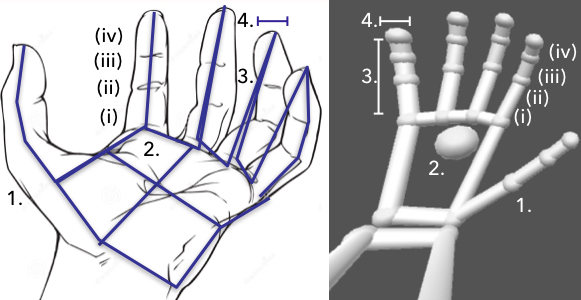
\includegraphics[width=1.0\textwidth]{Chapter2/Figs/Figure2-5.png}
\caption[Example of LMC generated hand model]{Example of LMC generated hand model}
\label{fig:Example_of_LMC_generated_hand_model}
\end{figure}

\begin{figure}
\centering
\def\svgwidth{\columnwidth}

\end{figure}



Information retrieved from the hand scans are summarised in Table ~\ref{table: Relevant LMC readings}. The LMC is capable of acquiring numerous metrics relating to any presented hand. A combination of Figure ~\ref{fig:Example_of_LMC_generated_hand_model} and Table ~\ref{table: Relevant LMC readings} provides an overview of the metrics that are relevant to the proposed system. It must be stated that i-iv can be further explained as the acquired lengths and widths of each of these bones.

\begin{table}[h]
\caption{Relevant LMC readings}
\centering
 \begin{tabular}{|p{0.45\textwidth} | p{0.45\textwidth}|} 
 \hline
	\textbf{Readings} & \textbf{Bone} \\ [1ex] 
 \hline\hline 
 1.	Left/Right (Hand) & (i) Metacarpal \\[1ex]
 \hline 
 2.	Palm Width (Hand) & (ii) Proximal \\[1ex]
 \hline
 3.	Length (Fingers) & (iii) Intermediate \\ [1ex] 
 \hline
 4.	Width (Fingers) & (iv) Distal \\ [1ex] 
 \hline
 \end{tabular}
 \label{table: Relevant LMC readings}
\end{table}


All of the above information becomes relevant when attempting to authenticate users based on their hand-geometry. Although the LMC maintains great accuracy when gathering information regarding to the presented hand, the readings tend to differ depending on the position of the hand in relation to the LMC device itself. The readings show minimal discrepancy (see Chapter 4); however, this could become an issue when statistically analysing the false acceptance rate and false rejection rate of the final authentication system \citep{Nagar2009}.

While scanning the hand using an LMC one can vary the length of the scans to acquire a larger data set for each user reading during the enrolment and storage phase. This allows for the system to iterate through the hand and its 19 bones (three bones per finger, except for the intermediate bone which is non-existent in the thumb) within the fingers and retrieve the lengths of each of those bones.

With the use of an LMC, features can be extracted from presented hands, transformed to implement CB and stored using steganography techniques. A proposed framework to implement such a system is discussed in the following section.


\section[Chapter summary]{Chapter summary}

The aim of this chapter was to provide sufficient background and insight into the various techniques that are to be used throughout the implementation of the cancelable biometric authentication system. The concepts and techniques that were explained will be used in the chapters that follow. Cancelable biometrics (along with the secure hashing standard), steganography and the use of the leap motion controller were explained with comparisons between different implementations thereof. This was done in order to select the best suited method that combines all the techniques in a manner that achieves secure storage of users’ hand geometry by using steganography.
Chapter 3 serves as a basis for the decision making process prior to the system implementation and offers the necessary literature to support the chosen techniques.



%!TEX root = ../thesis.tex
%*******************************************************************************
%****************************** Third Chapter **********************************
%*******************************************************************************
\chapter{System design}

% **************************** Define Graphics Path **************************
\ifpdf
    \graphicspath{{Chapter3/Figs/Raster/}{Chapter3/Figs/PDF/}{Chapter3/Figs/}}
\else
    \graphicspath{{Chapter3/Figs/Vector/}{Chapter3/Figs/}}
\fi

\section{Introduction}

The literature and background seen in Chapter 2 are used as a basis for the decision making throughout the design and development phase of this cancelable biometric authentication system. 
In order to successfully implement a biometric authentication system, there are various fundamental characteristics that need to be taken into consideration (as seen in Section). With these characteristics in place, only then is one able to amend the necessary techniques of cancelability and steganography in an attempt to provide a suitable working model for testing and evaluation. 
This chapter serves as a guide to the process followed during the design and development of the cancelable biometric authentication system and how the various techniques were implemented in this particular study.


\section{Process overview}

Due to the nature of the study, it is necessary to ensure that the development of the cancelable biometric authentication system should follow certain protocols that pertain to the techniques of cancelability and steganography. The relevant knowledge attained throughout the literature review (Chapter 2) clarified the manner within which the system would be developed. During the design and development phase of this system, various increments occurred to allow for the continuous integration of the vast features correlating to each individual technique. Thus, the system development adopted the iterative and incremental model. This model will now be further discussed. The aforementioned increments will now be discussed in more detail.

\section{SDLC - Iterative and incremental model}

This approach methodically attempts to develop software by gradually increasing functionality through planning multiple increments that produce deliverables. Each deliverable produced should ultimately contribute to the completed system (REFERENCE). 


% Figure - Iterative and incremental model
    
    \begin{figure}[htbp!] 
    \centering    
    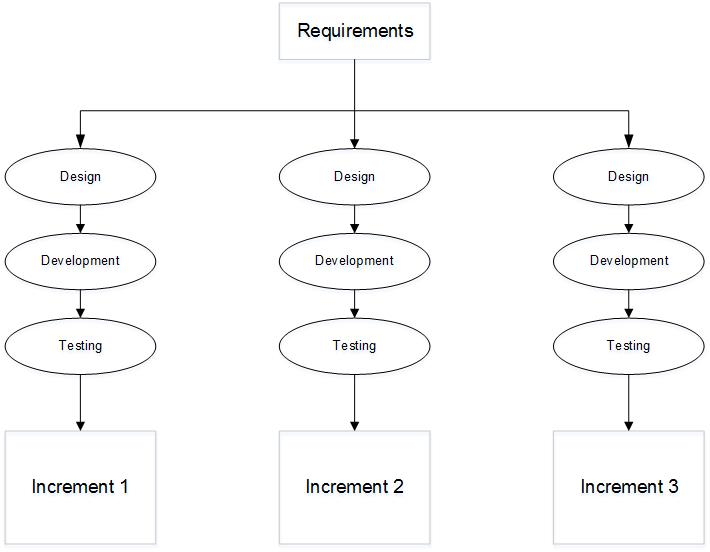
\includegraphics[width=1.0\textwidth]{Chapter3/Figs/Iterative_and_Incremental_Model.jpg}
    \caption[Iterative and incremental model]{Iterative and incremental model}
    \label{fig:Iterative and incremental model}
    \end{figure}
    
By using this method, the proposed authentication system was initiated through the use of a detailed planning process that involved mapping out the various goals for each increment of development. The goals for each increment included appending functionality to the previous increment. It was determined early on that by reaching these smaller goals and ensuring that the system functionality for each increment is met, the final system integration would be rudimental. The holistic approach is of utmost importance when developing a system using multiple increments. Due to the nature of the requirements that were set out in the early stages of research, the final authentication system would have to be constructed in a fashion. As seen in chapter 2, various techniques are required to function as expected to within their own regular circumstances before they can be implemented, tested and integrated to the final system. 
The iterative and incremental model is one that is based on producing deliverables. To illustrate the planning that went into the development of this final system, the Figure ~\ref{fig:Requirements} is presented and discussed. 

% Figure - Requirements
    
    \begin{figure}[htbp!] 
    \centering    
    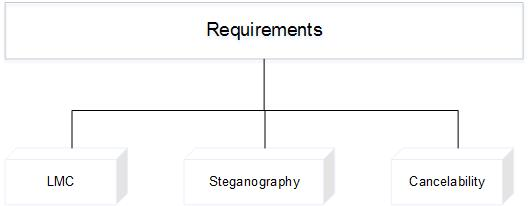
\includegraphics[width=1.0\textwidth]{Chapter3/Figs/Requirements.jpg}
    \caption[Requirements]{Requirements}
    \label{fig:Requirements}
    \end{figure}    
    
    The way in which the requirements for this project were setup and maintained largely had to do with the final system in mind. From the inception of this study, it was decided that the final authentication had to function in the following ways:
    
    \begin{enumerate}[label=\roman*.]
    	\item With the use of an inexpensive, functional peripheral device and an authentication sensor to provide a user-friendly and affordable solution to biometric readers;
    	\item The system would have to use a novel approach to storing biometric information obtained from the aforementioned sensor; and
    	\item Due to the novelty of the biometric storage, the system users’ biometrics should not be vulnerable to impersonation attacks.
    \end{enumerate}
    
With the functionality of the final authentication system established, the increments for the development were rendered transparent. As seen in the Figure ~\ref{fig:Development life cycle for proposed authentication system}, the increments for the project would evolve around meeting three main requirements, namely:

    \begin{enumerate}[label=\roman*.]
        \item Use the leap motion controller as the authentication sensor and ensure that it can read user hands efficiently and accurately;
        \item Apply steganographic techniques as a storage mechanism for the biometric reading provided by the leap motion controller; and
        \item Ensure that the users original biometric readings are safely stored using the abovementioned techniques and are mathematically irreversible.
    \end{enumerate}
    
   % Figure - Development life cycle for proposed authentication system
    
    \begin{figure}[htbp!] 
    \centering    
    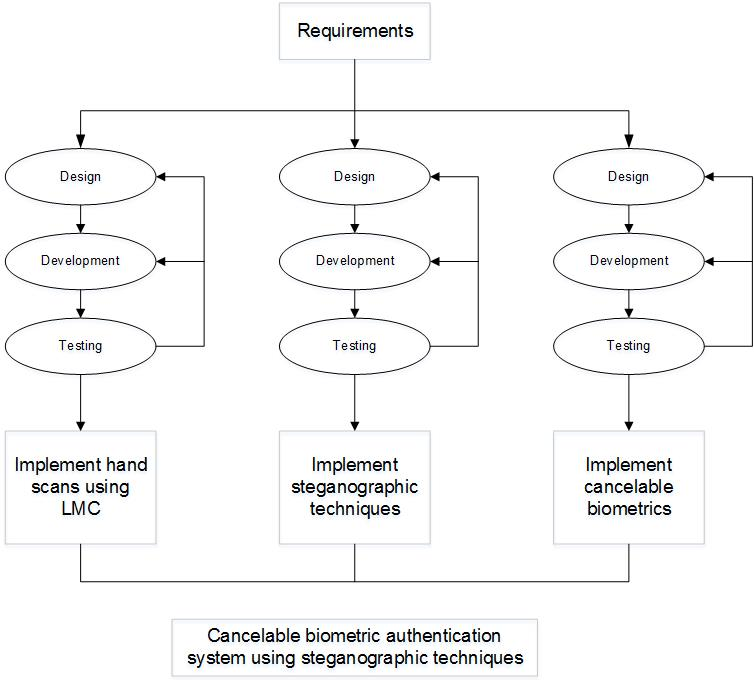
\includegraphics[width=1.0\textwidth]{Chapter3/Figs/Development_Cycle_for_Proposed_Authentication_System.jpg}
    \caption[Development life cycle for proposed authentication system]{Development life cycle for proposed authentication system}
    \label{fig:Development life cycle for proposed authentication system}
    \end{figure}
    
	
The development process will be discussed in more detail regarding each increment and its iterations.
By using these requirements to guide the development process, the first increment was instantiated by attempting to learn how the leap motion controller can be used to extract more information regarding a user’s hand. For this, the developer documentation was consulted regarding the setup thereof.

\section{System design flow / Proposed framework}

The prevailing architectures of biometric authentication systems consist of two main phases. These phases involve enrolment and authentication. The reason these two phases are required is so that during the authentication phase, the system has a biometric to compare to the biometric currently being presented to the system. This comparative biometric is typically referred to as a biometric template. During the enrolment phase, the biometric template is created for the user and then stored in a database. The manner within which the biometric template is created consists of several images being taken of the hand and then algorithmically extracting features from those images to create a final model for the specified user [19]. This entire enrolment phase can be simplified through the use of an LMC due to its ability to extract hand features from the internal LMC hand model that is created upon presentation of the hand. In order to comply with CB practices, this hand model has its features transformed mathematically, such that the original biometric information is not used in the transit/storage processes. The authentication phase simply compares the presented hands’ extracted features to those of the models within the database. This authentication process would, therefore, also need to transform the presented biometrics in order to match it to the stored model.

Figure ~\ref{fig:System structure flowchart} represents the information (system structure) flow within the authentication system. The LMC initiates the information flow for the system when the hand is presented and immediately extracts features therefrom. Once the features are extracted, they can be transformed mathematically allowing for the enrolment phase to commence. In an attempt to further secure the biometric information, the decision was made to implement two-factor authentication. This is done by issuing a 4-digit PIN to each new user that is enrolled into the system. For implementation purposes, the use of 4-digit PINs allows for a maximum unique user capacity of nine thousand users (randomly generated and numbered from 1000 to 9999). The issued user PIN will determine where in the stego-image the biometric information is stored. By taking this approach, the system is then able to use two different images for storage (one for PINs and one for the biometrics). 

% Figure - System structure flowchart
    
    \begin{figure}[htbp!] 
    \centering    
    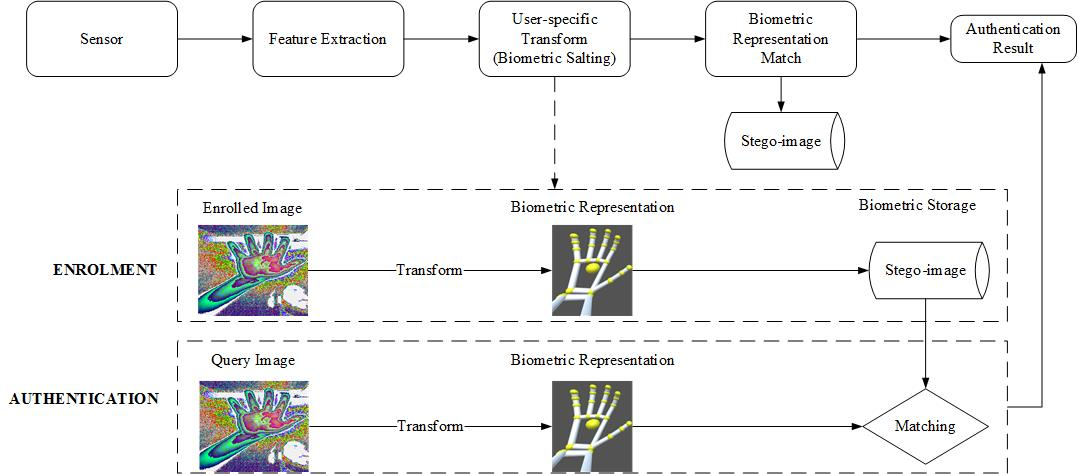
\includegraphics[width=1.0\textwidth]{Chapter3/Figs/System_Structure_Flowchart.jpg}
    \caption[System structure flowchart]{System structure flowchart}
    \label{fig:System structure flowchart}
    \end{figure}
    
In order to generate stego-images for sensitive information storage, one needs to specify exactly what images are made up of, how they are processed and how to programmatically generate them.

\section{System development process}


\subsection{LMC development}

As seen in the Figure ~\ref{fig:System structure flowchart}, the overall system structure flow is initiated through the feature extraction through the use of a sensor. In this particular study, the sensor refers to the leap motion controller. To successfully extract features from the user, the LMC needs to be setup according to the particular environment that will be used throughout the development. 

The environment chosen for the study was based on prior knowledge, the level of support documentation provided by Leap Motion and available resources in order to minimize the amount of time taken to learn and adapt to novelties. 

\subsubsection{LMC development environment}

In order to reiterate the manner within which the LMC functions, it is important to refer back to the API documentation for reference. For the purposes of feature extraction regarding the peripheral device, the hand detection can be summarised as follows:

Distance recorded by the LMC is measured in millimetres. 
To successfully extract accurate measurements pertaining to each individual hand that is presented to the LMC a Cartesian coordinate system is employed. 	This particular coordinate system manages to specify the various planes associated to the X, Y and Z-axes with regards to their orientation relative to the LMC device. This can be seen in Figure ~\ref{fig:LMC device structure and orientation}. 

% Figure - Randomly generated image versus stego-image
    
    \begin{figure}[htbp!] 
    \centering    
    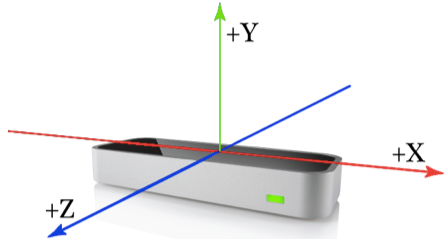
\includegraphics[width=1.0\textwidth]{Chapter3/Figs/LMC_device_structure_and_orientation.png}
    \caption[LMC device structure and orientation]{LMC device structure and orientation}
    \label{fig:LMC device structure and orientation}
    \end{figure}


The LMC generates infrared light, along with the use of optical sensors that originate directly from the centre, on top of the device. The Y-axis directs the sensors upwards and provides values that are incremented positively, contrasting to the downward orientation of the majority of computer graphics coordinate systems. The X and Z-axes lie on the horizontal plane of the LMC device with the X-axis positioned along the horizontal face of the device. The Z-axis provides positive values that increment toward the user. 

To provide further context as to how the LMC will be used to extract useful biometric information relating to the presented user hand, the following architecture allows a visual representation of the measurements that will be extracted during a scan. It is important to note that the LMC is capable of extracting far more information than what will be used in this particular study. The information and measurements relevant to this study include (and are limited to) the following information that can all be obtained from within the Hand object. The Hand object can further drill down into Finger objects. These Finger objects can then provide more information depending on the finger type. Each finger type then provides Bone objects that list the bone type correlating to the specific finger type. From those bone types, we are then able to measure those particular bones.  As provided by the developer API documentation on Leap Motion’s website, the Figure ~\ref{fig:LMC presented hand objects during extraction} provides a visual representation of how the hand object can be matched to suit the needs of this study.

% Figure - Randomly generated image versus stego-image
    
    \begin{figure}[htbp!] 
    \centering    
    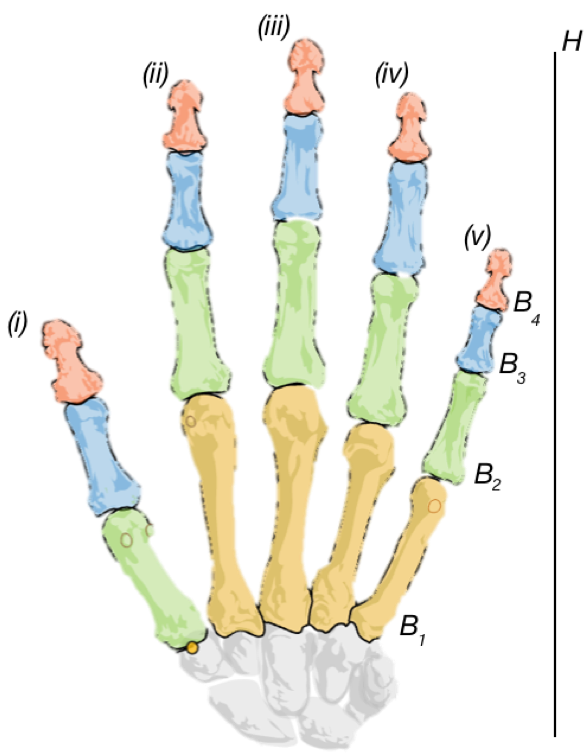
\includegraphics[width=8cm,height=9cm,keepaspectratio]{Chapter3/Figs/LMC_presented_hand_objects_during_extraction.png}
    \caption[LMC presented hand objects during extraction]{LMC presented hand objects during extraction}
    \label{fig:LMC presented hand objects during extraction}
    \end{figure}

In Figure ~\ref{fig:LMC presented hand objects during extraction}, it is of relevance to present the corresponding information relating to the objects.

%  Table - LMC hand object mapping according to infrared scan


    \begin{table}[h!]
    \caption{LMC hand object mapping according to infrared scan}
    \centering
     \begin{tabular}{|p{0.3\textwidth} | p{0.3\textwidth}| p{0.3\textwidth}|} 
     \hline
    	\textbf{Object} & \textbf{Symbol} & \textbf{Name} \\ [1ex] 
     \hline\hline 
     Hand & \textit{H} & Hand Class  \\
     \hline 
     \multirow{5}{*}{Finger} & \textit{(i)} & Thumb \\

            & \textit{(ii)} & Index     \\
     
            & \textit{(iii)} & Middle     \\
     
            & \textit{(iv)} & Ring     \\
     
            & \textit{(v)} & Pinky      \\
    \hline        
    \multirow{4}{*}{Bone} & \(B_1\) & Metacarpal\\
     
            & \(B_2\) & Proximal phalanges     \\
     
            & \(B_3\) & Intermediate phalanges     \\
     
            & \(B_4\) & Distal phalanges     \\
     \hline
     \end{tabular}
    \end{table}
    
With the guidance of the API documentation provided by Leap Motion, one was able to classify all of the necessary information into a model that is easier to understand during the development process. 

With the use of the above table, it was evident what the class hierarchy would have to be in order to successfully implementing the extraction of hand geometry measurements. The information would then be further classified using a Unified Modeling Language to visiualise the object structure to be used in the extraction algorithm.

Once the model has been set out and the measurements have been extracted from the presented user hand we can then prepare the extracted biometric for transformation. However, prior to transformation we must consider where the biometric will be stored and what the template will be. For this we need to prepare the storage using steganographic techniques. In the following section, the stego-image’s and how they were generated will be discussed.

\renewcommand{\umltextcolor}{black}
\renewcommand{\umldrawcolor}{black}
\renewcommand{\umlfillcolor}{white}

\begin{center}
\begin{tikzpicture}

\begin{class}{ Hand }{0 ,0}
    \attribute{ isRight : Bool }
    \operation{ CheckHand (  )}
\end{class}

\begin{class}{ Finger }{ 0 , -5}
    \inherit{ Hand }
    \attribute{ fingerType : String }
    \operation{ CheckFingerType ( )}
\end{class}

\begin{class}{ Bone }{0 , -10}
    \inherit{ Finger }
    \attribute{ boneType : String }
    \operation{ CheckBoneType ( ) }
\end{class}

\end{tikzpicture}
\end{center}


To aid the development process, Leap Motion has presumed the thumb metacarpal to have a length of 0.
This process all occurs at the time of initiating the scan via the LMC. To further illustrate the function used in the development of the extraction process, the following Algorithm ~\ref{algorithm: Leap motion controller algorithm to extract hand geometry} can be consulted.
    


%******************************************************************************************

% Algorithm - Leap motion controller algorithm to extract hand geometry

\begin{algorithm}[H]
 \SetKwInOut{Input}{Input}
    \SetKwInOut{Output}{Output}

    \underline{function ExtractHandGeometry} $(hand)$\;
    \Input{Hand object}
    \Output{Hand Measurements ($fingerLength$, $boneLength$)}
    \For{$hand$ in $hands$}{
        \eIf{$hand$=$RightHand$}{
            \For{$finger$ in $Fingers$}{
                \DontPrintSemicolon
                \space
                $fingerType$ = ClassifyFinger($finger$); 
                \tcp{Thumb, Index, Middle, Ring \& Pinky}
                
                \Switch{$fingerType$}{
                    
                
                    \For{$bone$ in $finger$}{
                        $boneType$ = ClassifyBoneType($finger$);
                        
                        \Switch{$boneType$}{
                            \tcp{Metacarpal, Proximal, Intermediate \& Distal }
                                AddMeasurements($boneType$);
                            
                        }
                    }
                }
                     
            }
            return $HandGeometryMeasurements$;
          }
          {
            return $CloseConnectionError$;
          }
    }
         
    \label{algorithm: Leap motion controller algorithm to extract hand geometry}
    \caption{Leap motion controller algorithm to extract hand geometry}
\end{algorithm}



To explain the Algorithm ~\ref{algorithm: Leap motion controller algorithm to extract hand geometry}, the first check that has to be done is one of what hand it is. Once the hand is confirmed to be the right hand, the algorithm can then proceed to check the fingers of that hand. Upon classification of the finger, the bones of that finger are then checked. Upon classification of the bone type, within the finger, within the hand, the measurement can be stored in a list. This process occurs for each hand upon enrolment of the finger (prior to storage) and upon authentication to match the measurements.

This research includes the use of the technique of creating cancelable biometrics. The first transformation of the hand geometry occurs within the scan of the hand, whether it be during enrolment or authentication. What is done to the original measurement initiates the cancelability. During the initial ten second enrolment scan, the measurements are extracted as previously discussed in Algorithm ~\ref{algorithm: Leap motion controller algorithm to extract hand geometry}. However, before storage, all of the measurements that have been temporarily been stored in a list are then aggregated for each of the nineteen bones. This total is then divided by the number of measurements that were taken by the LMC during the scan. The average measurement for each bone is then stored in an array of nineteen unique measurements that are rounded off to the nearest zero. This array of nineteen measurements is then transformed for the first time into a vector of five unique values (one for each finger). This vector is 5 values is the first line of defence in protecting the users biometric. The manner within this Algorithm ~\ref{algorithm: Transform algorithm} can protect the biometric has to do with the transformation that takes place to form this new 5 value vector. For this example, the values are mathematically transformed by simply aggregating the bone measurements within each finger. It should be noted that any mathematical function can be applied at this point. However, for simplicity, the values are merely aggregated. 

Another technique can be applied at this point to practice cancelability by simply discarding particular bone measurements ensure that the cancelability is reusable (as mentioned in Chapter 2). By simply changing the way in which the measurements are transformed mathematically can add value to ensuring cancelability. 

An illustrative example will clarify this process towards the end of this section.

%******************************************************************

The above Algorithm ~\ref{algorithm: Leap motion controller algorithm to extract hand geometry} adds every user's hand geometry measurements to a list. This list consists of +-10 000 readings.

Once these readings have been recorded and stored during the initial scan, the Algorithm ~\ref{algorithm: Create user hand geometry during enrolment} to drill-down into meaningful hand geometry measurements takes place. This Algorithm ~\ref{algorithm: Create user hand geometry during enrolment} can be seen below.

For each of the bones, in each of the fingers, on each of the hands, the measurements are aggregated. Once the measurements for each finger and it's bones are extracted, this Algorithm ~\ref{algorithm: Create user hand geometry during enrolment} iterates through the stored readings, aggregates the values, calculates the average (aggregated readings/number of readings), rounded off to the nearest integer. Once this vector is created, the vector is then further transformed. 

%Algorithm - Create user hand geometry vector during enrolment

\begin{algorithm}
     \SetKwInOut{Input}{Input}
    \SetKwInOut{Output}{Output}
    \underline{function EnrolUser} $(HandGeometryMeasurements)$\;
    \Input{All of the different hand geometry measurements (Finger and Bone Lengths)}
    \Output{HandGeometry vector}
    \tcc{This is used to keep track of the number of readings taken during the scan for each finger/bone scan}
    $counter$; 
    \tcc{This is an average measurement calculated for each finger and bone as mentioned above.}
    $measurementAverages$; 
    \For{$value$ in $measurements$}{
        $measurementAverage$ += value;
    }
    $measurementAverage$ = \textit{RoundToNearestZero($measurementAverage/counter$)}
    \For{$measurementAverage$ in $HandGeometryMeasurements$}{
        \tcc{This refers to each of the 19 bone measurements and individual finger measurements extracted during the initial scan, as mentioned in explanation of bone structure within the hand.}
        $vector$ = \textit{ArrayOfMeasurements($measurementAverage$)}
        
    }
    \tcp{This is the transformed vector from the array of measurements, passed through the final \textit{transformVector} function}
        $transformedVector$ = transformVector($vector$);
    return $transformedVector$
    
    \label{algorithm: Create user hand geometry during enrolment}
    \caption{Create user hand geometry vector during enrolment}
\end{algorithm}


\subsection{Steganographic development}

%Algorithm - Create stego-image for PINS

\begin{algorithm}
     \SetKwInOut{Input}{Input}
     \SetKwInOut{Output}{Output}
     
     \underline{function CreatePINStegoImage} ()\;
     \Output{$randomImage$}
     
     \textbf{Array} $allPins$ = \textbf{CreateUserPins(9000)}\;
     
     \For{$pin$ in $allPins$}{
        GenerateHash($pin$)\;
     }
     
     \textbf{int} $length$ = $allPins$.Length\;
     
     $height$ = 90\;
     $width$ = 800\;
     
     Bitmap $randomImage$ = new Bitmap($width$, $height$)\;
     
     \For{(\textbf{int} y = 0; y < $height$; y++)}{
     
        \For{(\textbf{int} x = 0; x < $width$; x++)}{
        
            \For{\textbf{int} i = i < $length$; i += 4}{
            
                $a$ = $allPins$[i]\;
                $r$ = $allPins$[i + 1]\;
                $g$ = $allPins$[i + 2]\;
                $b$ = $allPins$[i + 3]\;
                
                $randomImage$.SetPixel(x, y, ARGB($a$, $r$, $g$, $b$))\;
            }
        
        
        }
     
     }
     
     return $randomImage$.Save()\;
     
     \label{algorithm: Create stego-image for PINs}
     \caption{Create stego-image for PINs}
\end{algorithm}

%******************************************************************
    %Create stego PIN image explanation
%******************************************************************
Before being able to apply steganographic techniques into this research, it was important to gain some knowledge regarding working with images and how they are composed. The first thing to note was how pixels store information. The main concept behind working with pixels was the manner in which the data would be stored within the image in order to accurately represent a user’s hand geometry, while maintaining the privacy thereof. 

In order for this particular system to work, it had to be thoroughly planned and mathematically accurate to avoid any complications. With the original plan being to use multifactor authentication with the use of 4-digit PINs, the manner within which these PINs are stored had to remain consistent and secure. Not only would the PINs have to be stored using steganography, but all of the users hand geometry that corresponded to each of those PINs as well. 

It was decided to incorporate use a type of mapping technique that would have two separate stego-images. By mapping out the user PINs for both stego-images, it provided an easy way to map and keep track of the users and where their information was stored. 

Initially, the random 4-digit PINs needed to be generated and mapped to the corresponding pixels. The way this was done involved some intricate calculations that had to be tested and verified various times before the stego-images were successfully generated. 

Firstly, stego-image 1 would contain the random 4-digit PINs after they had been hashed using the SHA-256 algorithm that was discussed in Chapter 2. The calculations went as follows:
The SHA-256 algorithm, as the name implies, produces a hash value consisting of 256bits. 
By using this algorithm for each of the PINs, we would have to specify what the bits per pixel (bpp) would have to be for each of the pixels within the stego-image. It was decided that 32bpp would be acceptable to use. 

Typically, what the bpp does is determine the number of colours that can be stored within an image. This number of colours that are in an image depend on the bpp value. This value grows exponentially. An example of this would be: 

If 1bpp = 2 colours and 2bpp = 4 colours, then 32bpp = 4294,967,296 colours. This is only relative due to the stego-images using the format of 32bpp to store the hashed values within the A, R, G and B values (8 bits each).

Furthermore, as seen in the Algorithm ~\ref{algorithm: Create 4-digit user PINs}, the values for the stego-images are generates at 90 X 800, providing a resolution of 7200. This is simply because of the amount of users that can have a unique 4-digit PIN given to them of 9 000. This means that each users information will be mapped and stored to 8 specific pixels within the stego-images. 

%******************************************************************

% Algorithm - Create 4-digit user PINs

\begin{algorithm}
     \SetKwInOut{Input}{Input}
     \SetKwInOut{Output}{Output}
     
     \underline{function CreateUserPINs} ($numberOfUsers$)\;
     \Input{$numberOfUsers$}
     \Output{$userPins$}
     
     List $userPins$ \;
     
     \While{$numberOfUsers$ <= 9000 \&\& !$userPins$.Contains()}
     {
        $userPins$.Add(Random(1 000, 10 000))\;
        $numberOfUsers$++\;
     }
     
     return $userPins$\;
     
     \label{algorithm: Create 4-digit user PINs}
     \caption{Create 4-digit user PINs}
\end{algorithm}

%******************************************************************
    %create 4 digit PIN explanation
%******************************************************************
The importance of generating the 4-digit PINs randomly and assigning the users with these PINs is to provide better suited mapping capabilities. It should be noted that if this system were to be scaled, it could easy be done by simply generating 5-digit PINs which would take the total number of users that the system could handle from 9000 to 90000.

When generating the 4-digit PINs that will be allocated to the users it is imperative that there following criteria are met:

\begin{enumerate}[label=\roman*.]
    \item No repeating PINs;
    \item 9000 unique PINs are generated;
    \item Unordered sequence (pseudo-random); and
    \item PINs are only generated once.
\end{enumerate}





Due to the abovementioned criteria, the PINs carry larger weight when applying them as multifactor authentication to the user along with his/her biometric. 

As described above, to meet the criteria for the PINs, it was decided to use PINs that start with 1. By doing so the number of PINs decreases from a possible 10000 to 9000. It was found uncommon for users to use PINs that start with a zero. 

The number of unique PINs can be verified using the following formula:
\begin{gather}
    N =  x^{n}    
\end{gather}


Where x is the number relating to the range of possible values that are considered. In this instance it would be 0 – 9, therefore x = 10. However, because we are only considering values that start with 1 and upward, the formula can be rewritten as follows:

\begin{gather}
    N = a^{n}.b^{n}.c^{n}.d^{n}    
\end{gather}


Where N is the number of possible unique values and a, b, c and d are the positions within the 4-digit PIN. In this particular example, a only has 9 possible values ranging from 1 to 9, whereas b, c and d can range from 0 to 9. This produces the equation:

\begin{gather}
    N = 9^{1}.10^{1}.10^{1}.10^{1} 
    = 9000    
\end{gather}



To calculate the probability of another user being able to guess your PIN, we would need to look at the statistical formula: 
\begin{gather}
    P (A) = \frac{Number of favourable outcomes}{Total number of possible outcomes}
\end{gather}


Where the probability of event A in this instance is 
\begin{gather}
    \frac{1}{9000} = 0,000111111.
\end{gather}

With the probability as low as this enhanced by the biometric feature transformation added to it, the likelihood of guessing a PIN and matching the biometric is very close to zero.

%******************************************************************
%Algorithm -  Create stego-image for users

\begin{algorithm}
     \SetKwInOut{Input}{Input}
     \SetKwInOut{Output}{Output}
     \underline{function CreateUserStegoImage} ($bitmap$, $bytes$)\;
     \Input{$bitmap$};
     \Output{$userAddedBitmap$};
     \tcp{Depending on the x, y coordinates associated to pin}
     \eIf{$bitmap$.GetPixels(x,y) == \textbf{populated}}{
        return Error\;
     }{
        \For{(\textbf{int} i = 0; i < 32; i += 4 )}{
        $userAddedBitmap$ = $bitmap$.SetPixel(x, y, ARGB($bytes$[i], $bytes$[i + 1], $bytes$[i + 2], $bytes$[i + 3]))\;
        }
     }
     return $userAddedBitmap$
     
     \label{algorithm: Create stego-image for users}
     \caption{Create stego-image for users}
\end{algorithm}

%******************************************************************
    %create stego-image 2 explanation
%******************************************************************

Initially, stego-image 2 is generated as a blank image with zero values for each pixel. The resolution of stego-image 2 is required to stay consistent with that of stego-image 1 in order to ensure uniformity during the enrolment and authentication phases. The above Algorithm ~\ref{algorithm: Create stego-image for users} occurs during the enrolment phase where admin rights should be displayed in order to add a user to the system. Upon enrolment, the system will allocate a PIN to the user. Once the PIN has been allocated to the user, the system will then attempt to populate the transformed geometry into the 8 pixels that are mapped in the same position of the PIN in stego-image 1. General error checking is shown in the Algorithm ~\ref{algorithm: Create stego-image for users}, but due to the transformed hand geometry being hashed using SHA-256, the bytes will be set accordingly into the specified pixels. When the user attempts to authenticate using the system, another scan will occur, the hand geometry will be transformed once more and then matched according to the new hash value.

\subsection{Stego-image contextualisation}

An image can be seen as a two-dimensional matrix that is made up of pixels containing information about the colours within each particular pixel. This pixel information can be used to store sensitive biometric information. Using steganography techniques to store the transformed biometric models in an image involves that in order to store these models, each models’ bit-data would have to be processed. All electronic information is essentially made up of 1’s and 0’s (or bits). This means that the models that are generated need to be manipulated in such a manner that each user model’s bit data can be extracted for processing thereof. Once this bit data is processed, it can then be stored within an image to correspond to a particular user. 

With two-factor authentication being applied, both the PIN and the hand geometry need to be stored. Using one image to store the PIN, the system can then use the stored PIN to enrol/locate a user in a second image. This can be likened to a one-to-one relational database model. To illustrate this concept, Table II shows how PIN information in the first image can be used to correspond to the hand geometry stored in the second image. For instance, in the first block of Table II, the bold number (1) represents the user ID slot number while 3648 is the user PIN. The corresponding slot in the second stego-image is then used as the storage location for the user hand geometry data.

%  Table - Stego-image 1: User IDs vs their pixel correlation (10 IDs x 8 pixels per ID x 5 rows


    \begin{table}[h!]
    \caption{Stego-image 1: User IDs vs their pixel correlation (10 IDs x 8 pixels per ID x 5 rows}
    \centering
     \begin{tabular}{|p{0.075\textwidth} | p{0.075\textwidth}| p{0.075\textwidth} | p{0.075\textwidth} | p{0.075\textwidth} | p{0.075\textwidth} | p{0.075\textwidth} | p{0.075\textwidth} | p{0.075\textwidth} | p{0.075\textwidth} |} 
     
     \hline
     \begin{minipage}{.075\textwidth}
      
\includegraphics[width=\linewidth, height=5mm]{Chapter3/Figs/TablePixels.jpg}
    \end{minipage}& & & & & & & & & \\[1ex]
     \textbf{1}, & \textbf{2}, & \textbf{3}, & \textbf{4}, & \textbf{5}, & \textbf{6}, & \textbf{7}, & \textbf{8}, & \textbf{9}, & \textbf{10},  \\[1ex]
     3648 & 7896 & 5091 & 4948 & 3102 & 7500 & 1651 & 6765 & 6865 & 7677  \\[1ex]
     
     \hline 
     \textbf{11}, & \textbf{12} & \textbf{13} & \textbf{14}, & \textbf{15}, & \textbf{16}, & \textbf{17}, & \textbf{18}, & \textbf{19}, & \textbf{20},  \\[1ex]
    5153 & 1782 & 2922 & 2183 & 1817 & 6372 & 1621 & 8283 & 2845 & 6931  \\[1ex]
     
     \hline
     \textbf{21}, & \textbf{22}, & \textbf{23}, & \textbf{24}, & \textbf{25}, & \textbf{26}, & \textbf{27}, & \textbf{28}, & \textbf{29}, & \textbf{30},  \\[1ex]
    2608 & 3587 & 6231 & 5373 & 3594 & 1877 & 3867 & 1080 & 2807 & 6143  \\[1ex]
     
     \hline           
     \textbf{31}, & \textbf{32}, & \textbf{33}, & \textbf{34}, & \textbf{35}, & \textbf{36}, & \textbf{37}, & \textbf{38}, & \textbf{39}, & \textbf{40},  \\[1ex]
     7362 & 4162 & 8075 & 8742 & 7851 & 3653 & 8431 & 4352 & 1238 & 2128  \\[1ex]
     
     \hline
     \textbf{41}, & \textbf{42}, & \textbf{43}, & \textbf{44}, & \textbf{45}, & \textbf{46}, & \textbf{47}, & \textbf{48}, & \textbf{49}, & \textbf{50},  \\[1ex]
    7673 & 2513 & 8825 & 5110 & 5701 & 6623 & 5963 & 1703 & 3697 & 2073  \\[1ex]
     
     \hline
     
     \end{tabular}
    \end{table}
    


%******************************************************************************************

In order to standardize the amount of data that can be used to store information within the pixels, the system uses 32bpp (bits per pixel) image formatting. This ensures that within each pixel of the image, 32 bits of information can be held. These 32 bits are made up of A (8 bits), R (8 bits), G (8 bits), and B (8 bits) values. Due to the fact that the number of bits used to store a 4-digit PIN would vary depending on the value, it was decided to also standardize the number of bits used during PIN storage per user. To do so, a hash-function is used [20]. 
The hash-function ensures that regardless of what the PIN is, the length of the hash representation will be similar. A SHA256 (Secure Hashing Algorithm 256-bit) function was chosen. This is because it is the successor of SHA1, which was compromised [21], and addresses the issues prevalent in SHA1.
Each PIN is made up of 256-bits (8 pixels, if one pixel = 32bpp), leading to 8 pixels to store user their information within both images. Referring back to the earlier statement of using two images with a one-to-one relationship, a user PIN can be mapped and correlated directly to the hand geometry in the second image using the hash function prior to enrolling the user.

Table II is an example illustration of user ID slots in correlation to the image pixels with an image resolution of 80 X 5. The first image is used to store hashed user PINs. 
To generate the stego-image, the PINs are shuffled to ensure that the PIN-ID combination is not sorted such that PIN 1000 is stored in the first 8 pixels using the ID slot 1 etc.

\subsection{Random PIN generation}

To counter the threat of reverse-engineering the generated PINs, a program was written that generated 9 000 (unsorted) unique 4-digit PINs and mapped each PIN to an ID that ranged from 1-9000. An example of such a mapping is demonstrated using Table II to illustrate that PIN 3648 correlates to the user ID of 1. With this information generated and stored locally, using a conversion to bit data, stego-image 1 was generated so that all of the hashed PINs were stored and mapped. Stego-image 1 will, thus, remain unaltered after it has been generated. Stego-image 2 can then be altered during the enrolment phase. This is further explained below.

\subsection{Stego-image generation}

Stego-image 2 is a randomly generated image that will be altered as users enrol into the system. During the enrolment phase, users will be issued a PIN. Depending on the PIN he/she receives, a user ID correlating to that PIN is known by the system. Once the system has calculated the user ID based on the PIN that was entered by the user, the pixels within stego-image 2 can be altered using the hashed hand geometry of the enrolling user. By altering stego-image 2 in this way using stego-image 1, the authentication phase become more efficient because the pixels containing the biometric information can be directly read due to the mapping. The authentication process would be inefficient if the system had to search through the entire image each time a user presented their hand. Since an image can be seen as a matrix with 9 000 users, the complexity to compare and authenticate the presented hand geometry to the image would be O(n²) each time. 

In order to gain a better understanding of how the system operates, the pseudo-code for the system is discussed.

\subsection{Cancelable biometric development}

%Algorithm - Transform algorithm

\begin{algorithm}
     \SetKwInOut{Input}{Input}
     \SetKwInOut{Output}{Output}
     
     \underline{function TransformVector}($ArrayOfMeasurements$)\;
     \Input{$ArrayOfMeasurements$}
     \Output{$transformed vector$}
     
     \For{$measurementAverage$ in $ArrayOfMeasurements$}{
        $transformedVector$ += $measurementAverage$\; 
        \tcp{Aggregated measurements for this example} 
     }
     
     return $transformedVector$\;
     \label{algorithm: Transform algorithm}
     \caption{Transform algorithm}
\end{algorithm}


%Algorithm - Generate Hash Algorithm
\begin{algorithm}
     \SetKwInOut{Input}{Input}
     \SetKwInOut{Output}{Output}
     
     \underline{function GenerateHash} ($transformedVector$)\;
     \Input{$transformedVector$}
     \Output{$vectorHash$}
     
     \textbf{\textit{using} SHA-256}{
        $hash$ = ComputeHash($transformedVector$)\;
        
        \For{$byte$ in $hash$}{
            $vectorHash$.add($byte$)\; 
        }
    
     }
     return $vectorHash$;
     \label{algorithm: Generate hash algorithm}
     \caption{Generate hash algorithm}
\end{algorithm}

%******************************************************************
    %generate hash output explanation
%******************************************************************

The SHA-256 algorithm was discussed in detail in Chapter 2. However, it has been added in here for completeness in order to provide context for how the bytes will be stored within the stego-images. 

The transformed vector that is passed into this function comes in the form of a text representation subsequent to the extraction scan that takes place from the LMC device. This will be further demonstrated in the following section that discusses the illustrative example.


\subsection{Pseudocode for system algorithm}

Keeping in mind the abovementioned information flow, as well as the mapping and stego-image generation, this pseudo-code should verify the exact functioning of the authentication system.
The pseudo-code below (Algorithm ~\ref{algorithm: Pseudocode for system algorithm}) aims to provide an overview of what input is retrieved within the system and to clarify how the two phases of biometric systems are applied based on the input retrieved from the user. As seen above, if the user is enrolled, the system merely transforms the presented hand geometry and authenticates the user by comparing the transformed information to that stored in stego-image 2.

%  Algorithm - Pseudocode for system algorithm

\begin{algorithm}
     \SetKwInOut{Input}{Input}
     \SetKwInOut{Output}{Output}
     
     \underline{function cancelableTransform($PIN$, array[] $fingerBoneInfo$)}\;
     \Input{$PIN$, $Biometric Features$ {handID (hID), array[boneType (bT), boneWidth (bW), boneLength (bL)]}}
     \Output{User-specific HashID for Steganography}
     
      \eIf{(PIN == hID) \&\& (enrolled == true)}{
        handGeo = Transform(fingerBoneInfo)\;
        Authenticate(getPixels(map),handGeo)\;
      }{
        newUser = Transform(fingerBoneInfo)\;
        EnrolUser(PIN, newUser)\;
      } 
        
      return HashID\;
     
     \label{algorithm: Pseudocode for system algorithm}
     \caption{Pseudocode for system algorithm}
\end{algorithm}

%*********************************************************

%******************************************************************
    %pseudocode explanation
%******************************************************************

The pseudocode for the entire system algorithm attempts to summarise the process that the authentication system follows, from the the initial scan during enrolment, to the matching of the transformed biometric that is presented by the user during authentication. 

This Algorithm ~\ref{algorithm: Pseudocode for system algorithm} describes the logic behind the system in a simplified manner to portray the main functionality. 

%******************************************************************


However, if the user has not been enrolled, he/she then is issued a PIN and the presented hand geometry is transformed and stored within stego-image 2, correlating to the issued PIN location.

Next, the advantages and disadvantages of the system will now be discussed.

\subsection{Advantages/Disadvantages}

The use of the current implementation of this authentication system has its advantages and disadvantages.


Advantages of the proposed system include:
    \begin{enumerate}[label=\roman*.]
        \item The low-cost factor; 
        \item Ease of use and convenience;
        \item The security aspects are superior when compared to passwords because authentication is based on a combination of PIN and hand information that cannot be stolen or guessed; and
        \item Auditability in terms of being able to connect users to a specific event or activity.
    \end{enumerate}
	
The disadvantages include: 
    \begin{enumerate}[label=\roman*.]
        \item The technology is still in its infancy and is not mature;
        \item While system performance for authentication is expected to be high for small organizations, it may pose a problem should more users need to be enrolled; and finally
        \item Error incidence due to changes in a person’s hands due to injury, old age, or illness.
    \end{enumerate}

The following section will provide an illustrative example of the system.

\section{Illustrative example}

In this section, a simplified example of a user being authenticated is presented in order to provide a holistic view to the combination of the topics discussed in previous sections.
With each hand that is presented to the LMC a model is created that is either used for enrolment or for authentication. Assuming that the user-hand that is presented has already undergone enrolment, the LMC will create a model using a particular transform parameter to compare this model to the binary representation of the hand already stored within stego-image 2. By using the PIN that is entered prior to hand scanning, the system ensures that the users’ transformed biometric representation can efficiently be compared to the newly transformed model. This is efficient because the system has mapped the PINs to pixel IDs, rather than having to search the entire image for the corresponding biometric representation.

Consider the explanation of the illustrative example shown in Figure ~\ref{fig:Example of biometric vector reading and transformation}.

% Figure - Example of biometric vector reading and transformation
    
    \begin{figure}[htbp!] 
    \centering    
    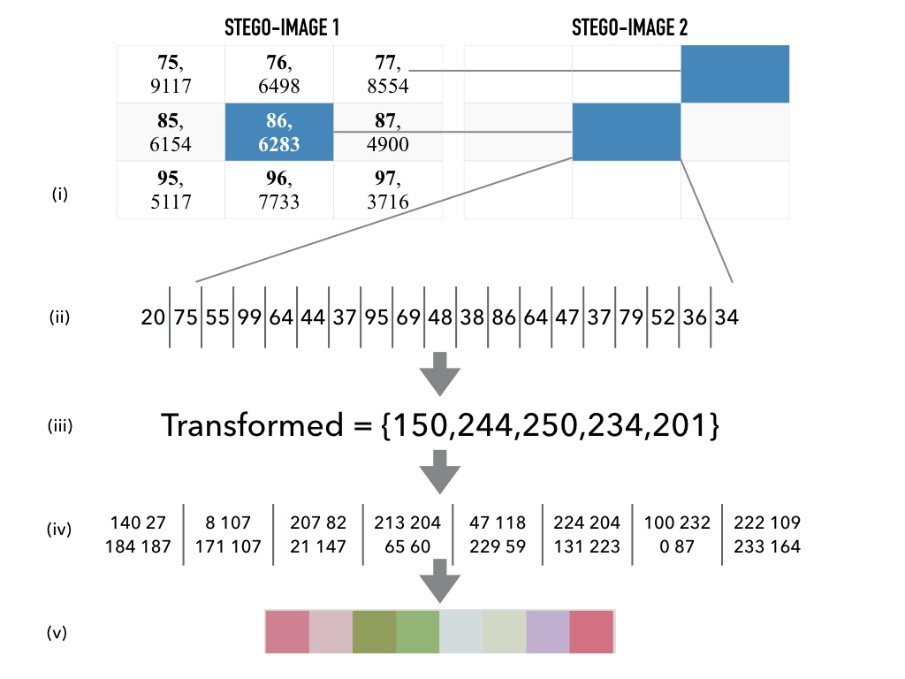
\includegraphics[width=1.0\textwidth]{Chapter3/Figs/Example_of_biometric_vector_reading_and_transformation.jpg}
    \caption[Example of biometric vector reading and transformation]{Example of biometric vector reading and transformation}
    \label{fig:Example of biometric vector reading and transformation}
    \end{figure}

\begin{enumerate}[label=\roman*.]
    
    \item  Assume the user was presented with the PIN 6283 during enrolment. The user would then have a dedicated storage section with the ID of 86 in both stego-image 1 and in stego-image 2. During the authentication phase the user will have his/her hand geometry scanned to compare the presented hand to the binary representation stored within stego-image 2. 
    
    \item  During the abovementioned scan, the hand geometry of the user is mathematically generated by using various combinations from the thousands of readings gathered to form one vector (readings for each of the 19 individual bones in his/her hand).
    
    \item By using the vector created in (ii), the system then transforms the biometric vector once more in order to implement CB (as discussed in Section II-A). In this particular example, the vector was simply transformed by adding each finger’s bone readings together (3 readings for the thumb and 4 readings for all the other fingers). It should be noted that more complex mathematical transformations are recommended for the actual implementation.
    
    \item The system further protects the biometric information by applying a SHA256 hash function to the vector. This vector is then represented as a byte array consisting of 32 values from the 256-bit hash function. Ultimately, this ensures that each user only uses 8 pixels within both the stego-images.
    
    \item Once the byte array has been generated, it can then be compared to the stored biometric representation within ID 86 consisting of 8 pixels.
Upon completion of the abovementioned process, the system will either accept the user as successfully authenticated, or the system will reject the user and ask for the hand to be re-scanned.

\end{enumerate}

By using steganography techniques, the system ensures imperceptibility and cancelability.

The Figure ~\ref{fig:Randomly generated image versus stego-image} provides a comparative view of two generated images for their use in this context. 

% Figure - Randomly generated image versus stego-image
    
    \begin{figure}[htbp!] 
    \centering    
    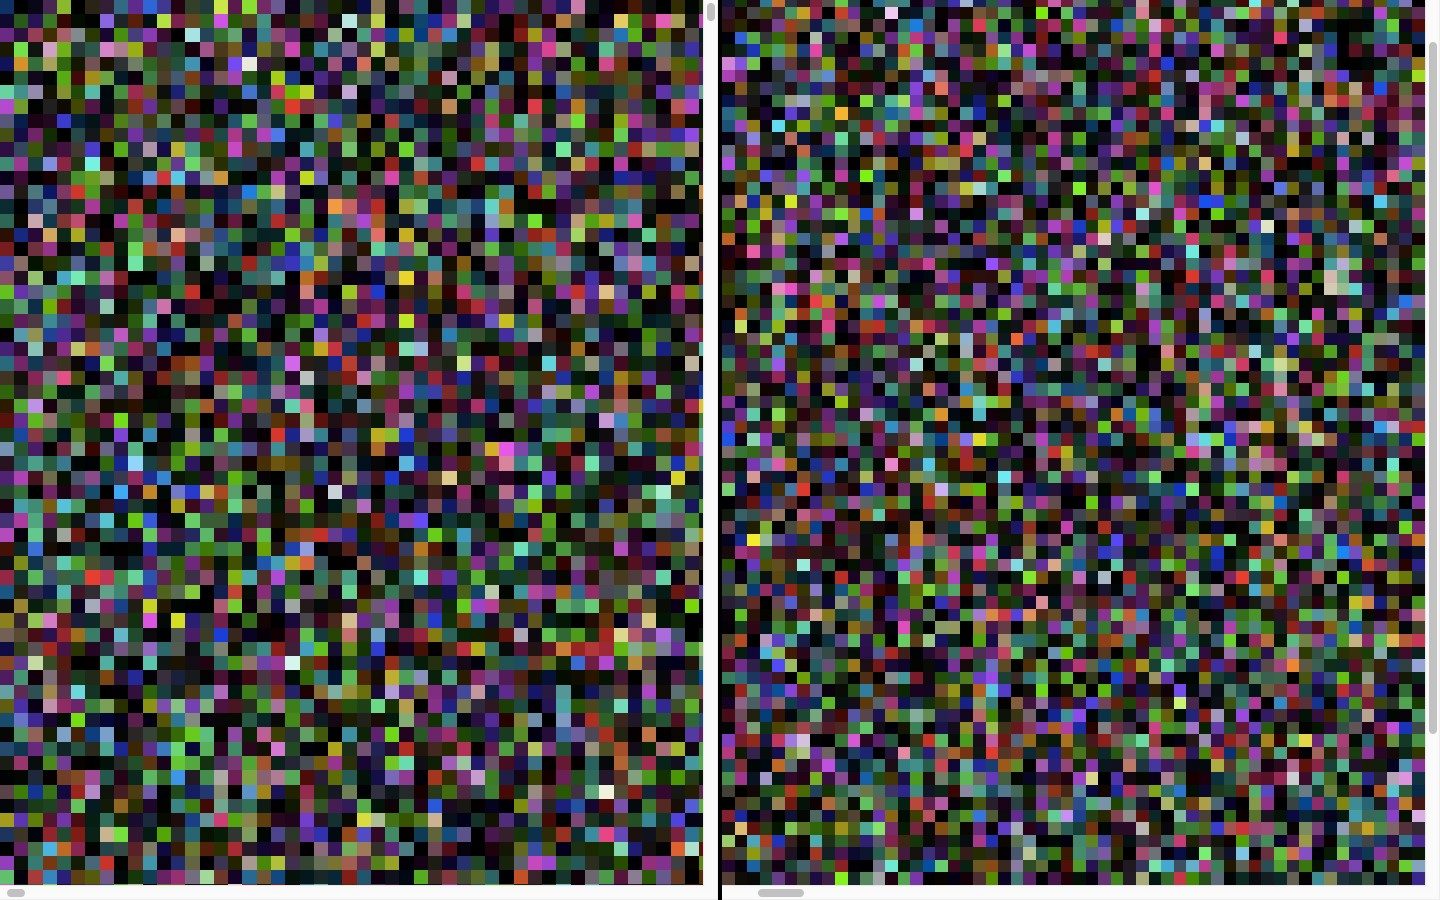
\includegraphics[width=1.0\textwidth]{Chapter3/Figs/Randomly_generated_image_versus_stego-image.jpg}
    \caption[Randomly generated image versus stego-image]{Randomly generated image versus stego-image}
    \label{fig:Randomly generated image versus stego-image}
    \end{figure}

The image on the left was randomly generated, while the image on the right contains sensitive biometric information. To the human eye one cannot easily infer that these two images differ, however, upon closer inspection one may realize differing colour mappings but cannot differentiate between sensitive data and just another randomly generated image.

Ultimately, cancelability can be concluded due to the biometric information being transformed and obscured prior to storage. This means that should an attacker find these two images in a compromised system, he/she will not know what information was used to generate these images, nor how the information was transformed prior to storage. In fact, without prior knowledge he/she will not even know to expect hidden data in said images.




% \section{Uncertain}

% Algorithm - check vector hash combinations

% \begin{algorithm}
%      \SetKwInOut{Input}{Input}
%      \SetKwInOut{Output}{Output}
     
%      \underline{function VectorCombinationsCheck} ( $transformedVector$, $count$)\;
%      \Input{$transformedVector$}
%      \Output{$result$}
     
%       \tcp{transformedVector, low and high are \textbf{arrays}}
%       $low$;
%       $high$;
     
%      $increment$ = 0;
     
%      \If{$count$ = $transformedVector$.Length}{
%         \textbf{return}\;
%      }
     
%      \For{($value$ in $transformedVector$)}{
%         $increment$++\;
        
%         \textbf{Array}.Copy($transformedVector$, $low$)\;
%         $low$[count] = $transformedVector$[count] - $increment$\;
%         \textbf{checkLowMatch} = GenerateHash($low$)\;
%         \textbf{Array}.Copy($transformedVector$, $high$)\;
%         $high$[count] = $transformedVector$[count] + $increment$\;
%         \textbf{checkHighMatch} = GenerateHash($high$);
%         \tcp{Recurse}
%         \textbf{VectorCombinationsCheck}($low$, count + 1)\;
%         \textbf{VectorCombinationsCheck}($high$, count + 1)\;
        
%      }
     
%      return $result$ = \textbf{VectorCombinationsCheck($transformedVector$)}
     
     
%      \caption{Recursive algorithm to find possible vector combinations}
% \end{algorithm}



\section{Conclusion}

\section{Chapter summary}





















%******************************************************************
    %template matching algorithm explanation
%******************************************************************

%TODO put in testing chapter 4

%!TEX root = ../thesis.tex
%*******************************************************************************
%****************************** Fourth Chapter **********************************
%*******************************************************************************
\chapter{Evaluation and data analysis}

% **************************** Define Graphics Path **************************

\section{Introduction}

In an attempt to quantify the performance of the proposed system, a threefold evaluation was instantiated and conducted. This is presented in terms of the consistency of the LMC, followed by a comparative vector tolerance analysis and finally, the overall system accuracy. Thereafter a discussion is presented. The following evaluation and discussion are based on sample data that was collected through the scanning (enrolment and authentication) of forty unique candidates.

\section{Testing methodology}

%****************************************************************

In testing the system, it was decided that a simulation should be initiated in order to determine the reliability and efficiency of the system by eliminating the LMC. This was done due to the device's lack of customisability. As the system stored the transformed biometric data of the forty users within stego-image 2, the simulation would attempt to authenticate only the user data that was extracted during enrolment and authentication phases. 

In order to successfully simulate the authentication process, the following steps would need to be conducted: 

\begin{enumerate}[label=\roman*.]
    \item Both stego-images will be stored to read information from within the test program
    \item A list will be created correlating to the users PINs;
    \item A list will be created correlating to the transformed hand geometry extracted during the authentication scans;
    \item These lists will be iterated accordingly having each PIN in the list hashed and matched to the data corresponding to that PIN in stego-image 1;
    \item Once the PIN has successfully matched, the corresponding authentication transformation will be hashed and matched to the data within stego-image 2;
    \item Each of the aforementioned steps will be timed in order to gauge the efficiency of the matching algorithm.
    
\end{enumerate}

% Figure - Simulation authentication test
    
    \begin{figure}[htbp!] 
    \centering    
    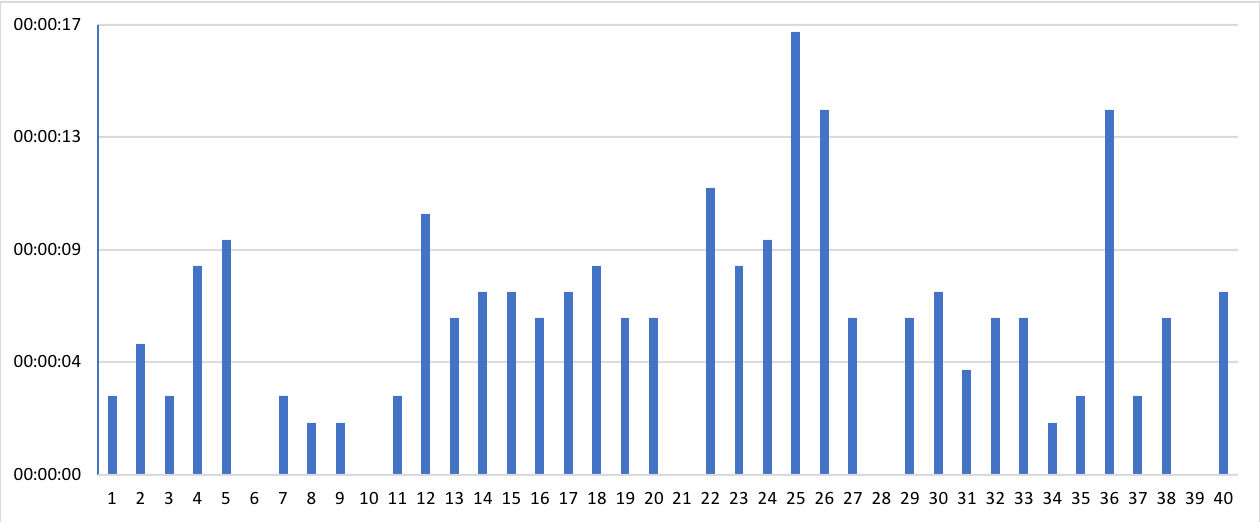
\includegraphics[width=1.0\textwidth]{Chapter4/Figs/AuthTest1.png}
    % \includesvg[width=0.8\textwidth]{Chapter4/Figs/AuthTest1.svg}
    \caption[Simulation for time taken to authenticate users]{Simulation for time taken to authenticate users}
    \label{fig:Simulation for time taken to authenticate users}
    \end{figure}
    
With the core functionality of the proposed system being to successfully transform and authenticate users, the efficiency is seen to be slightly lacking. As the above Figure \ref{fig:Simulation for time taken to authenticate users} shows, the algorithm used to find the authentication match within the threshold tolerance range of 5 affects the speed at which a user can be authenticated. A simple and effective solution to this drawback of obtaining a successful match may be to place an upper limit on the time that the algorithm is allowed to scan for a match for. This upper limit can be deduced from the average time taken to authenticate all forty users of 6,65s. 


\subsection{Leap Motion Controller performance evaluation}

To illustrate the efficiency and reliability of the LMC, the data that was collected from one randomly selected, five second hand geometry scan is presented in both Table~\ref{table: Randomly selected data from five second scan} and Figure~\ref{fig:Five Second hand scan graph} below. 
In order to present a visualisation with a high enough resolution to be able to see the variance in the scan readings, only the three fingers most similar in length are shown in Figure~\ref{fig:Five Second hand scan graph}(i.e., the index, middle, and ring fingers). 

% Table - Data from One, 5 second hand geometry scan
    
    \begin{table}[h!]
    \caption{Randomly selected data from five second scan}
    \centering
     \begin{tabular}{|p{0.18\textwidth} | p{0.18\textwidth}| p{0.18\textwidth}| p{0.18\textwidth}| p{0.18\textwidth}|} 
     \hline
    	\textbf{Thumb} & \textbf{Index} & \textbf{Middle} & \textbf{Ring} & \textbf{Pinky} \\ [1ex] 
     \hline\hline 
     0.197203783 & 0.424346553 &  0.464246258 & 0.438259197 & 0.35738522 \\[1ex]
     \hline 
     \end{tabular}
     \label{table: Randomly selected data from five second scan}
    \end{table}

% Figure - Five Second hand scan graph
    
    \begin{figure}[htbp!] 
    \centering    
    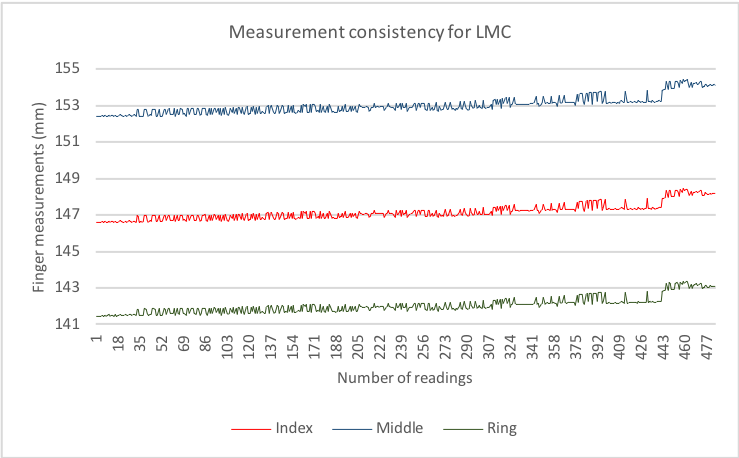
\includegraphics[width=1.0\textwidth]{Chapter4/Figs/Consistency.png}
    % \includesvg[width=0.8\textwidth]{Chapter4/Figs/Figure1.svg}
    \caption[Five Second hand scan graph]{Five Second hand scan graph}
    \label{fig:Five Second hand scan graph}
    \end{figure}
    
The significance of this data is prevalent when taking into consideration the distribution throughout the scan. It is of utmost importance to conistently extract concise data readings throughout the length of the scan. Thus, the standard deviation of the raw data correlating to the plotted data was calculated in an attempt to demonstrate the accuracy that the LMC provides (see Table~\ref{table: Randomly selected data from five second scan}).

It is interesting to note that the longer the scan has progressed, the more varied the readings become. This is attributed to the instability that is associated with an unsupported hand being held in mid-air for any given period of time.

\subsection{Comparitive vector tolerance}

Despite the above-mentioned LMC accuracy, the system shows slight deviation from one scan to the next. To provide an explicit limit regarding the deviation of the readings during a scan, it was decided to measure a tolerance range.

The manner within which this tolerance range was calculated involves comparing test data from user enrolment scan to that of the associated authentication scan. This data includes all of the users and their transformed vector combinations. With this data, the maximum tolerance range was extrapolated based on the variations produced by the system. As seen in Figure~\ref{fig:Comparative vector tolerance} below, it was concluded that the maximum tolerance range for this data set is 5mm.

% Figure - Comparative vector tolerance
    
    \begin{figure}[htbp!] 
    \centering    
    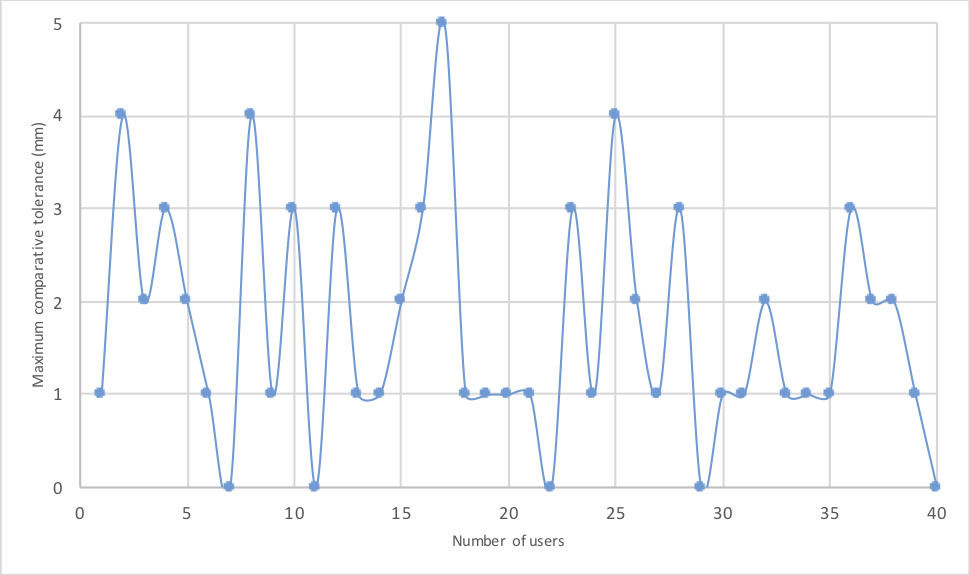
\includegraphics[width=1.0\textwidth]{Chapter4/Figs/Comparative.png}
    % \includesvg[width=1\textwidth]{Chapter4/SVG/Comparative-pdf.svg}
    \caption[Comparative vector tolerance]{Comparative vector tolerance}
    \label{fig:Comparative vector tolerance}
    \end{figure}

Upon further evaluation, with the tolerance range at a maximum of 5mm, the acceptance rates exponentially improved. This, however, increased the processing time to find a positive match within the tolerance range of the transformed vector. 

\section{Algorithm evaluation}

As with any authentication system, one needs to take into consideration human error or inconsistency during the scanning process. To better illustrate the thought process prior to the formulation of the Algorithm \ref{algorithm: Recursive algorithm to find possible vector combinations}, consider the following example:

\begin{enumerate}[label=\roman*.]
    \item User A enrols with the transformed hand geometry vector of {50, 60, 70, 80, 90};
    \item When the user A attempts to authenticate thereafter, his/her hand is not scanned identically due to various factors and the transformed hand geometry vector produced this time is {52, 59, 74, 81, 90}
    \item Due to the SHA-256 hashing applied to the transformed geometry prior to storage, the match to the value stored within stego-image 2 fails, even though user A has provided the correct PIN.
    \item In order to provide greater match accuracy, an algorithm was formulated in order to compensate for fault tolerance during scans.
    \item As seen in Figure \ref{fig:Comparative vector tolerance}, the fault tolerance was variable for a range of 5 for each vector value.
\end{enumerate}

With a fault tolerance of 5mm, the probability of finding an exact match of the stored biometric increases exponentially. Algorithm~\ref{algorithm: Recursive algorithm to find possible vector combinations} attempts to find a match as efficiently as possible while reducing the amount of false positive matches produced by the system.

Once the scanned vector is passed into this algorithm, the calculations proceed as follows:

\begin{enumerate}[label=\roman*.]
    \item The original transformed vector is copied and the 1st value is decremented by 1;
    \item This alteration creates a new vector;
    \item This vector is then hashed and compared to what is stored in stego-image 2.
    \item The process repeats itself for each value until the last value in the original vector is decremented by 1;
    \item The 1st value is then incremented by 1, hashed and compared to what is stored in stego-image 2;
    \item The process then repeats itself and increases the increment to 2, 3, 4 and 5 respectively;
    \item If a match is found during this process, the algorithm is halted. If no match is found, the algorithm continues to recursively search for a match until the possible vector combinations are exhausted.
\end{enumerate}

The above-mentioned process is illustrated below in Algorithm~\ref{algorithm: Recursive algorithm to find possible vector combinations}.
% Algorithm - check vector hash combinations

\begin{algorithm}
     \SetKwInOut{Input}{Input}
     \SetKwInOut{Output}{Output}
     
     \underline{function VectorCombinationsCheck} ( $transformedVector$, $count$)\;
     \Input{$transformedVector$}
     \Output{$result$}
     
      \tcp{transformedVector, low and high are \textbf{vectors}}
      $low$;
      $high$;
     
     $increment$ = 0;
     
     \If{$count$ = $transformedVector$.Length}{
        \textbf{return}\;
     }
     
     \For{($value$ in $transformedVector$)}{
        $increment$++\;
        
        \textbf{Array}.Copy($transformedVector$, $low$)\;
        $low$[count] = $transformedVector$[count] - $increment$\;
        \textbf{checkLowMatch} = GenerateHash($low$)\;
        \textbf{Array}.Copy($transformedVector$, $high$)\;
        $high$[count] = $transformedVector$[count] + $increment$\;
        \textbf{checkHighMatch} = GenerateHash($high$);
        \tcp{Recurse}
        \textbf{VectorCombinationsCheck}($low$, count + 1)\;
        \textbf{VectorCombinationsCheck}($high$, count + 1)\;
        
     }
     
     return $result$ = \textbf{VectorCombinationsCheck($transformedVector$)}
     
     \label{algorithm: Recursive algorithm to find possible vector combinations}
     \caption{Recursive algorithm to find possible vector combinations}
\end{algorithm}

This approach attempts to decrease the false-positive match rates. 

%****************************************************************

\subsection{Overall system evaluation}

As deduced from Figure~\ref{fig:System tolerance versus acceptance rates}, a 0mm tolerance rate resulted in only a 12.5\% true acceptance rate. If this tolerance is then increased, the true acceptance rate also increases (e.g. 97.5\% with a 4mm tolerance) until a 100\% true acceptance rate is obtained at 5mm tolerance. 
When considering implementing this particular system approach, one needs to determine what risk factor is suitable within the authentication scenario. If the users that need to be authenticated are to be granted access to sensitive data/areas, then the tolerance range should be adjusted accordingly. The acceptance rate is drastically affected when using the maximum tolerance range. With such a high tolerance range, the false acceptance rate is also dramatically increased, but because of the two-factor authentication provided with the allocated PIN, the users are authenticated correctly and no inter-user error is observed where one user is authenticated as another.

% Figure - System tolerance vs acceptance rates
    
    \begin{figure}[htbp!] 
    \centering    
    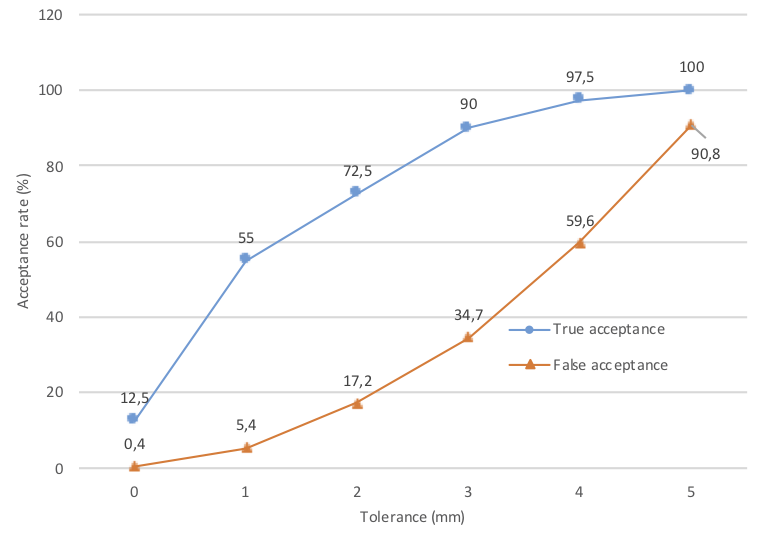
\includegraphics[width=1.0\textwidth]{Chapter4/Figs/Tolerance.png}
    % \includesvg[width=1\textwidth]{Chapter4/SVG/Tolerance-pdf.svg}
    \caption[System tolerance versus acceptance rates]{System tolerance versus acceptance rates}
    \label{fig:System tolerance versus acceptance rates}
    \end{figure}


\section{Discussion}

The proposed technique has revealed several promising advantages by using a combination of the techniques specified in Chapter 2. The LMC was found to be a stable and efficient hand geometry scanner. Also, the steganography techniques used in this paper were relatively easy to implement for use in this particular instance. By using PINs (to implement two-factor authentication) the security is enhanced and aids in achieving cancelability for storing biometrics. The proposed framework ensured that the system provided results that were reliable and efficiently obtained.

Bearing in mind the above-mentioned advantages, some disadvantages are present when using this approach. The algorithm to find positive matches slowed down the system. It may be of value to consider the possibility of removing the algorithm in future and alternatively producing a false match, followed by a re-scan. This system was only exposed to limited testing and the authentication accuracy and robustness will need to be measured using a formal evaluation. In order to fully explore the system’s functionality, extensive tests should be conducted upon this framework on a larger scale. This will form part of the ongoing research.


\section{Chapter summary}

The aim of this chapter was to evaluate the overall system design, performance, accuracy and efficiency. This was done by analysing data extracted during the testing process. Once analysis on that data was complete, the system performance, accuracy and efficiency was measured using simulation tests by removing certain system components. The algorithmic complexity was analysed for optimisation possibilities.

In Chapter 5, the objectives of the study will be revisited and discussed. Any problems experienced throughout the study will also be addressed and opportunities that may have come to fruition throughout the research will be discussed for future studies.
%!TEX root = ../thesis.tex
%*******************************************************************************
%****************************** Fifth Chapter **********************************
%*******************************************************************************
\chapter{Conclusion}

% **************************** Define Graphics Path **************************

\section{Introduction}

Chapter 5 aims to conclude this study by presenting definitive remarks and comments. The aforementioned will be based on the research objectives that were made concrete during the initial stages and whether or not these objectives were realised throughout the study. The limitations that arose will also be discussed, as well as new opportunities that have become apparent upon completion.

\section{Reflection}


\section{Research objectives}

In chapter 1, it was stated that in order to achieve the primary objective of this study, various secondary objectives would first need to be met. Thus, these objectives will be discussed first.


\textbf{Objective 1:} \textit{With the use of a literature review, discuss the use and implementation of cancelable biometrics, steganography, hand geometry authentication and the Leap Motion Controller.}


To address this objective, chapter 2 involved thorough research into a multitude of seemingly disparate techniques and attempting to unify them to provide a holistic approach for an authentication system. The discussions regarding these techniques focussed on their individual characteristics and what the best practices were for implementing each of those techniques independently. It was realised during the discussions within the literature review that these techniques could, in theory, collectively produce a framework that achieves an authentication system.


\textbf{Objective 2:} \textit{Design and implementation of the system}


Upon realisation that the collective techniques could produce an authentication system, the design and implementation of this proposed system would have to be laid out systematically. In chapter 3, the system design process was mapped out using the iterative and incremental approach which allowed us to materialise smaller “goals” or increments that needed to be implemented in order to successfully create the proposed authentication system. These increments guided the development process and it was ensured that the primary objective of this study was well aligned with the aforementioned increments. 

The implementation process presented various challenges that were overcome due to the knowledge that was gained throughout the literature review and was well managed through the use of the iterative and incremental model. Throughout the entirety of chapter 3, the development of the system was discussed, highlighting the crucial algorithmic functions that were needed in order to meet the incremental authentication system capabilities. By meeting this secondary objective, the only objective remaining would be to thoroughly test the functionality of the system.


\textbf{Objective 3:} \textit{Evaluation of the created system using error-based metrics and iterative validation testing}


In order to conclusively state that the proposed authentication system is fully functional, an evaluation of the system using error-based metrics and iterative validation testing would need to be done. This testing would be conducted in a manner that extracts data from multiple users in an attempt to:

\begin{enumerate}[label=\roman*.]
    \item Enrol the user into the system; and
    \item Successfully, accurately and efficiently authenticate the user.
\end{enumerate}

Once this data was collected during the testing and evaluation, a benchmark for the testing could be concluded in order to: 

\begin{enumerate}[label=\roman*.]
    \item Compare the efficiency and accuracy; and 
    \item Security of the proposed system.
\end{enumerate}

Upon thorough analysis of the extracted data, the results were then discussed and it was found that even though the system lacked efficiency and could be optimized to authenticate users faster, it did so with a high success rate and a high accuracy rate.


\textbf{Objective 4:} \textit{Develop a technique that ensures cancelability if biometrics based on hand geometry information from an LMC and steganographic storage techniques.}


The primary objective of this study was to develop a technique that ensures cancelability if biometrics based on hand geometry information from an LMC and steganographic storage techniques. As the abovementioned statement indicates, the proposed authentication system aimed to:

\begin{enumerate}[label=\roman*.]
    \item Extract biometric information (specifically hand geometry measurements) from users;
    \item Ensure that these biometrics are made cancellable using various techniques to transform the biometric information prior to storage; 
    \item Upon storing the cancellable biometrics, steganographic techniques will be used.
\end{enumerate}

Thus, it can be stated that all of the objectives, as described in chapter 1 and reiterated here, have been successfully addressed and achieved. In meeting these objectives, the possibilities surrounding affordable and secure authentications have surfaced. 


\subsection{Research assertion}

Biometric cancelability can be enhanced using user-based transform parameters (obtained from an LMC) for a steganography algorithm that stores biometric information.

\section{Contribution to field}

\subsection{Using the LMC in a new context}

\subsection{Using steganography in a new context}

\subsection{Ensuring cancelability for novel biometrics}

\section{Limitations}

With regards to the setup of the proposed framework, it must be stated that there were few limitations in terms of the actual development of the system due to the wide range of supported development platforms, languages and firmware. However, a limitation to the system remains that the LMC is a peripheral device and therefore requires a host to run on. The minimum system requirements for the system can be seen in Appendix C.
When the testing of the system came about, another limitation occurred in terms of the number of participants during testing. Due to the number of willing and available members within the computer science faculty at the NWU Potchefstroom campus, the total number of participants was capped at forty. 
Even though the LMC proved to be an effective an efficient biometric sensor, the use of hand geometry for the source of user biometric revealed the lack of uniqueness found in this approach. It might have been more useful to use a more distinctive biometric (such as fingerprints). However, with the reduced cost of using a peripheral device like the LMC, the limitations posed by this approach may also be seen as advantageous due to the ease of use and affordability.

\section{Future work}

The combination of techniques presented within this study are merely one approach that can be taken, and various other approaches may be taken to create an authentication system. Another possible approach that could be taken for future research may be to use fingerprints as the biometric source, along with an alternative CB approach, as well as, using steganography in a different way. The proposed system could open many possibilities into the manner within which cancelable biometrics are used within authentication systems.
Further studies may also include the use of a larger data set to provide more detailed analysis regarding the cancelability and accuracy of the proposed framework.

To improve the proposed framework, one could look at the vast number of opportunities that were revealed throughout the research process. Some of these opportunities involve: 


\begin{enumerate}[label=\roman*.]
    \item Improving the system performance by using more efficient search algorithms to match users faster;
    \item Increasing the level of security provided through the steganographic techniques by applying a greater level of dynamic randomness during the enrolment and storage process; 
    \item Using mathematically complex approaches to apply cancelability prior to the biometric storage and matching processes; and
    \item The system can be upgraded to use cloud services for storing the stego-images rather than storing the information locally.
\end{enumerate}

\section{Chapter summary}

Chapter 5 is the final chapter of this study and aimed to present a summary of the objectives that were presented in chapter 1 and how these objectives were approached and achieved. Therefore, the limitations that were realised throughout the study and the possibilities that arose upon completion thereof.
% %!TEX root = ../thesis.tex
%*******************************************************************************
%****************************** Sixth Chapter **********************************
%*******************************************************************************
\chapter{Conclusion}

% **************************** Define Graphics Path **************************

\section{Introduction}

Chapter 6 aims to conclude this study by presenting definitive remarks and comments. The aforementioned will be based on the research objectives that were made concrete during the initial stages and whether or not these objectives were realised throughout the study. The limitations that arose will also be discussed, as well as new opportunities that have become apparent upon completion.

\section{Research objectives}

In chapter 1, it was stated that in order to achieve the primary objective of this study, various secondary objectives would first need to be met. Thus, we will discuss these objectives first.

\subsection{With the use of a literature review, discuss the use and implementation of cancelable biometrics, steganography, hand geometry authentication and the Leap Motion Controller.}

To address this objective, chapter 2 involved thorough research into a multitude of seemingly disparate techniques and attempting to unify them to provide a holistic approach for an authentication system. The discussions regarding these techniques focussed on their individual characteristics and what the best practices were for implementing each of those techniques independently. It was realised during the discussions within the literature review that these techniques could, in theory, collectively produce a framework that achieves an authentication system.

\subsection{Design and implementation of the system}

Upon realisation that the collective techniques could produce an authentication system, the design and implementation of this proposed system would have to be laid out systematically. In chapter 3, the system design process was mapped out using the iterative and incremental approach which allowed us to materialise smaller “goals” or increments that we needed to implement in order to successfully create the proposed authentication system. These increments guided the development process and we ensured that the primary objective of this study was well aligned with the aforementioned increments. 

The implementation process presented various challenges that were overcome due to the knowledge that was gained throughout the literature review and was well managed through the use of the iterative and incremental model. Throughout the entirety of chapter 3, the development of the system was discussed, highlighting the crucial algorithmic functions that were needed in order to meet the incremental authentication system capabilities. By meeting this secondary objective, the only objective remaining would be to thoroughly test the functionality of the system.


\subsection{Evaluation of the created system using error-based metrics and iterative validation testing}

In order to conclusively state that the proposed authentication system is fully functional, we would have to evaluate the system using error-based metrics and iterative validation testing. This testing would be conducted in a manner that extracts data from multiple users in an attempt to:

\begin{enumerate}[label=\roman*.]
    \item Enrol the user into the system; and
    \item Successfully, accurately and efficiently authenticate the user.
\end{enumerate}

Once this data was collected during the testing and evaluation, a benchmark for the testing could be concluded in order to: 

\begin{enumerate}[label=\roman*.]
    \item Compare the efficiency and accuracy; and 
    \item Security of the proposed system.
\end{enumerate}

Upon thorough analysis of the extracted data, the results were then discussed and it was found that even though the system lacked efficiency and could be optimized to authenticate users faster, it did so with a high success rate and a high accuracy rate.

\subsection{Develop a technique that ensures cancelability if biometrics based on hand geometry information from an LMC and steganographic storage techniques.}

The primary objective of this study was to develop a technique that ensures cancelability if biometrics based on hand geometry information from an LMC and steganographic storage techniques. As the abovementioned statement indicates, the proposed authentication system aimed to:

\begin{enumerate}[label=\roman*.]
    \item Extract biometric information (specifically hand geometry measurements) from users;
    \item Ensure that these biometrics are made cancellable using various techniques to transform the biometric information prior to storage; 
    \item Upon storing the cancellable biometrics, steganographic techniques will be used.
\end{enumerate}

Thus, it can be stated that all of the objectives, as described in chapter 1 and reiterated here, have been successfully addressed and achieved. In meeting these objectives, the possibilities surrounding affordable and secure authentications have surfaced. 

\section{Limitations}

With regards to the setup of the proposed framework, it must be stated that there were few limitations in terms of the actual development of the system due to the wide range of supported development platforms, languages and firmware. However, a limitation to the system remains that the LMC is a peripheral device and therefore requires a host to run on. The minimum system requirements for the system can be seen in Appendix C.
When the testing of the system came about, another limitation occurred in terms of the number of participants during testing. Due to the number of willing and available members within the computer science faculty at the NWU Potchefstroom campus, the total number of participants was capped at forty. 
Even though the LMC proved to be an effective an efficient biometric sensor, the use of hand geometry for the source of user biometric revealed the lack of uniqueness found in this approach. It might have been more useful to use a more distinctive biometric (such as fingerprints). However, with the reduced cost of using a peripheral device like the LMC, the limitations posed by this approach may also be seen as advantageous due to the ease of use and affordability.


\section{Future research}

The combination of techniques presented within this study are merely one approach that can be taken, and various other approaches may be taken to create an authentication system. Another possible approach that could be taken for future research may be to use fingerprints as the biometric source, along with an alternative CB approach, as well as, using steganography in a different way. The proposed system could open many possibilities into the manner within which cancelable biometrics are used within authentication systems.
Further studies may also include the use of a larger data set to provide more detailed analysis regarding the cancelability and accuracy of the proposed framework.

To improve the proposed framework, one could look at the vast number of opportunities that were revealed throughout the research process. Some of these opportunities involve: 


\begin{enumerate}[label=\roman*.]
    \item Improving the system performance by using more efficient search algorithms to match users faster;
    \item Increasing the level of security provided through the steganographic techniques by applying a greater level of dynamic randomness during the enrolment and storage process; 
    \item Using mathematically complex approaches to apply cancelability prior to the biometric storage and matching processes; and
    \item The system can be upgraded to use cloud services for storing the stego-images rather than storing the information locally.
\end{enumerate}

\section{Chapter summary}

Chapter 6 is the final chapter of this study and aimed to present a summary of the objectives that were presented in chapter 1 and how these objectives were approached and achieved. Therefore, the limitations that were realised throughout the study and the possibilities that arose upon completion thereof.
% \include{Chapter7/chapter7}



% ********************************** Back Matter *******************************
% Backmatter should be commented out, if you are using appendices after References
%\backmatter

% ********************************** Bibliography ******************************
\begin{spacing}{1.5}

% To use the conventional natbib style referencing
% Bibliography style previews: http://nodonn.tipido.net/bibstyle.php
% Reference styles: http://sites.stat.psu.edu/~surajit/present/bib.htm

\bibliographystyle{agsm}
% \bibliographystyle{unsrt} % Use for unsorted references  
% \bibliographystyle{plainnat} % use this to have URLs listed in References
\cleardoublepage
\bibliography{References/AllMendeleyRefs} % Path to your References.bib file


% If you would like to use BibLaTeX for your references, pass `custombib' as
% an option in the document class. The location of 'reference.bib' should be
% specified in the preamble.tex file in the custombib section.
% Comment out the lines related to natbib above and uncomment the following line.

% \printbibliography[heading=bibintoc, title={References}]


% \nocite{*}
% \printbibliography[keyword=1]

\end{spacing}

% ********************************** Appendices ********************************

\begin{appendices} % Using appendices environment for more functunality

%!TEX root = ../thesis.tex
% ******************************* Thesis Appendix A ****************************
% \chapter{Publication at SecureWare Conference} 
% \section{Appendix A}

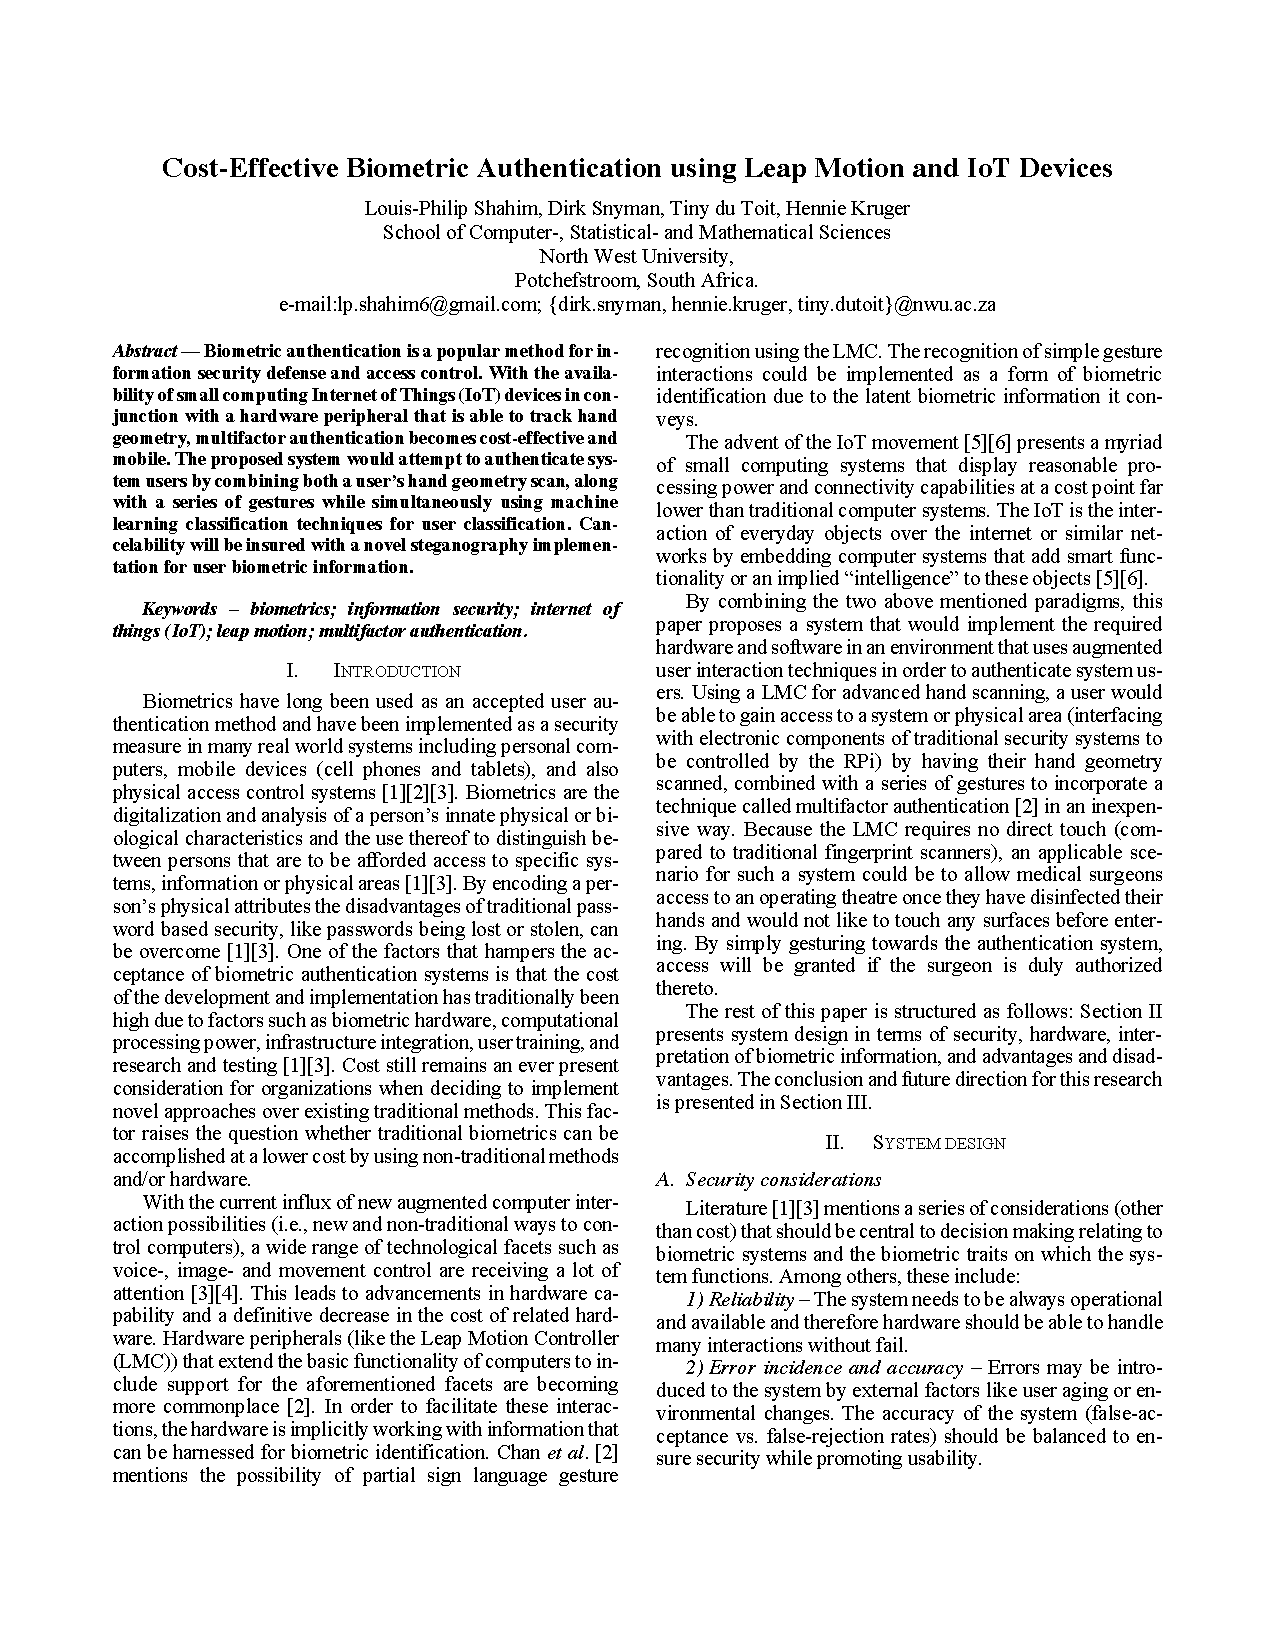
\includepdf[pages=1,scale=.8,pagecommand={\section{Appendix A}}]{Appendix1/Secureware.pdf}
\includepdf[pages=2-,pagecommand={}]{Appendix1/Secureware.pdf}
% %!TEX root = ../thesis.tex
% % ******************************* Thesis Appendix B ********************************

\chapter{IARIA}
\label{AppendixB}
\textbf{Journal paper published in The International Journal of Advances in Security} \\

The Internation Journal of Advances in Security publishes special issues, from time to time, that draws contributions from its sister conferences. Such contributions are selected by the editors of the journal based on the publications in the proceedings of the conferences. Based on the the relevance and recommendations from the peer review process, selected papers are invited to be extended for inclusion in the special issues of the journal.

The conference paper in Appendix A was selected for publication in the International Journal of Advances in Security and is subsequently presented here in Appendix B. The main results of the study were presented in this paper. Before publication, the paper subjected to a double-blind peer review.\\

\textit{Contributions of authors:}
\begin{itemize}
    \item[--] Shahim, Louis-Philip - Principle investigator and lead author
    \item[--] Snyman, Dirk - Supervisor and experimental design
    \item[--] Du Toit, Tiny - Co-supervisor and critical reader (technical)
    \item[--] Kruger, Hennie - Co-supervisor and critical reader (conceptual)
\end{itemize}

\textbf{Bibliographic reference:} Shahim, L.P.; Snyman, D.P.; Du Toit, J.V.; Kruger, H.A. Cancelable hand geometry-based biometric authentication system using steganography techniques. \textit{International Journal of Advances in Security}, 2017, 10, pp. 134-144.

% Paper published in the International Journal of Advances in Security 10 (3 \& 4), 134-144. This journal article was written under invitation to do so and was subject to peer review.

% This paper involved the bulk of the literature review and has been the greatest contribution to this particular study. The development of the proposed framework was primarily based on the findings mentioned here.

% This journal article was presented at the 44th ORSA conference in 2017. Valuable insights were gained from that conference and the necessary applications and adjustments were made to the study for the better.

% The final journal article can be seen on the pages that follow.

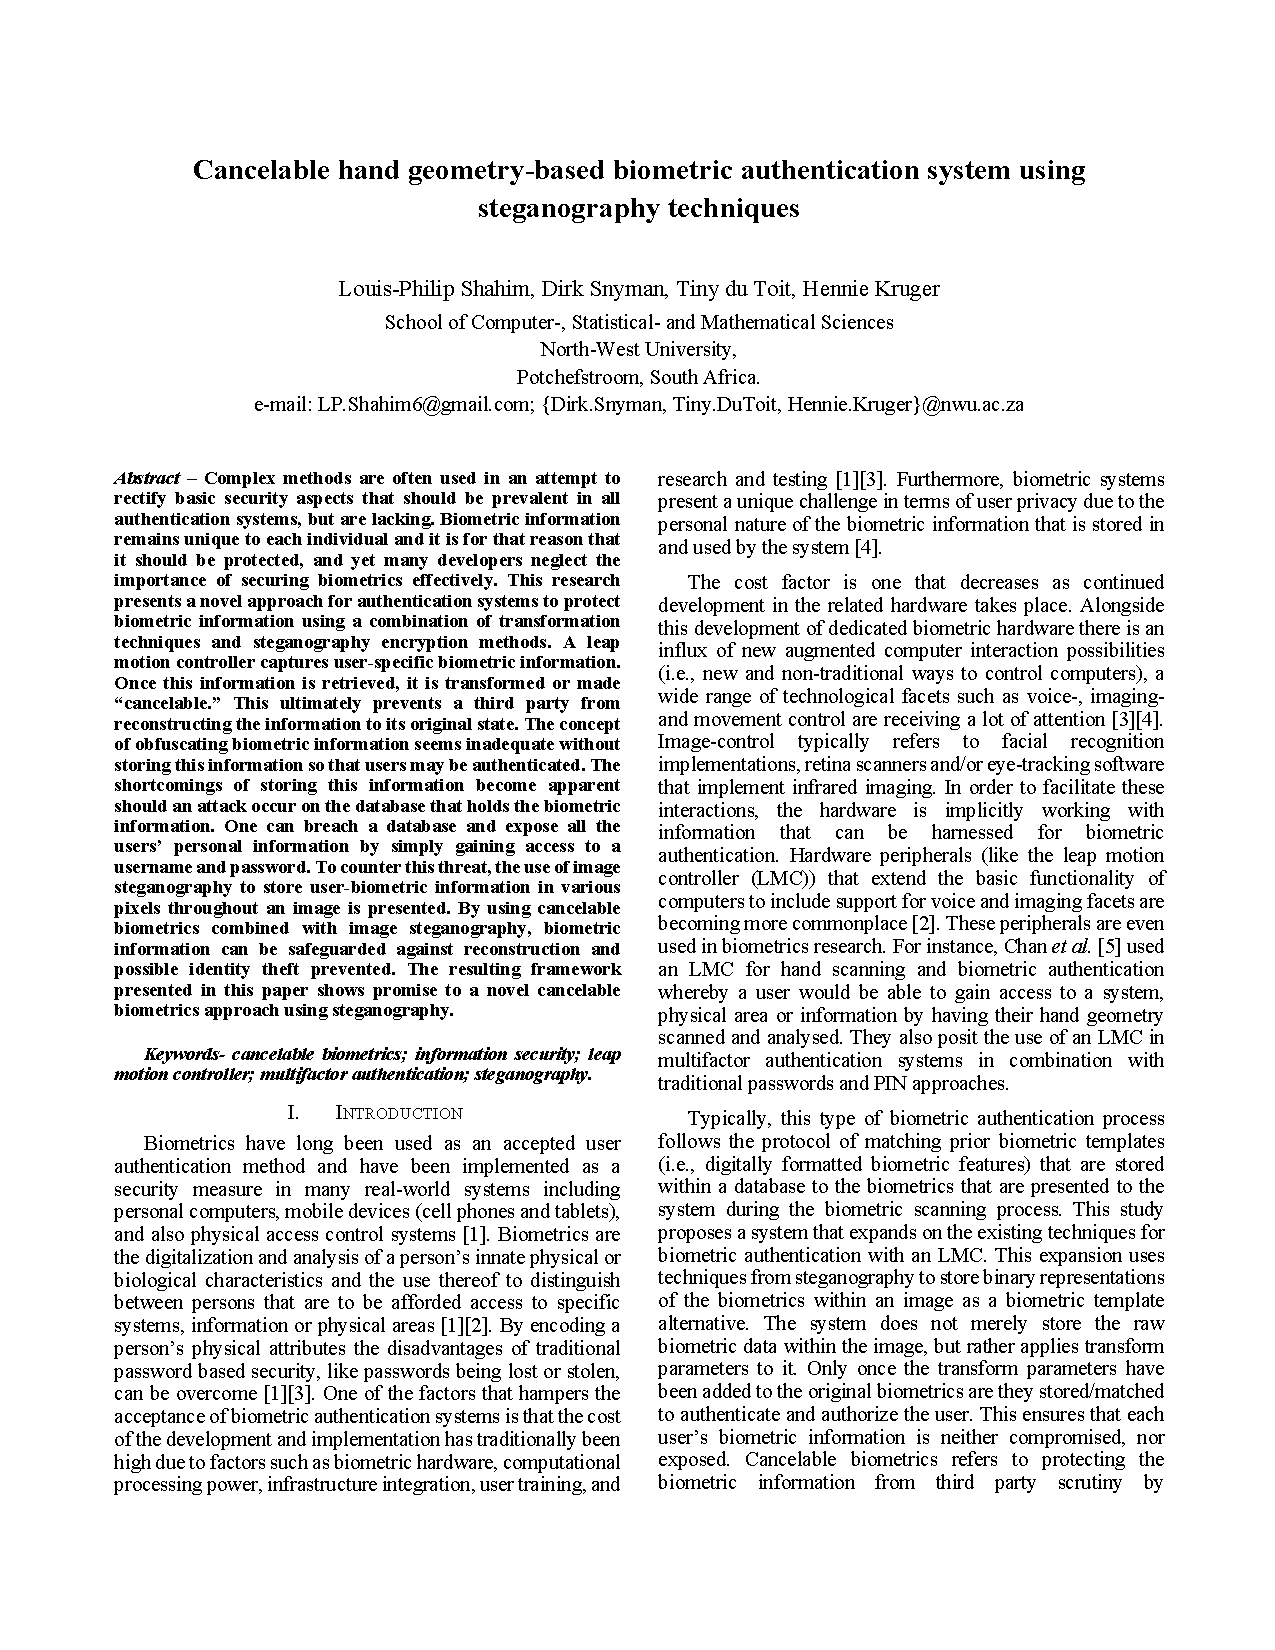
\includepdf[pages=1-,pagecommand={}]{Appendix2/IARIA.pdf}
% 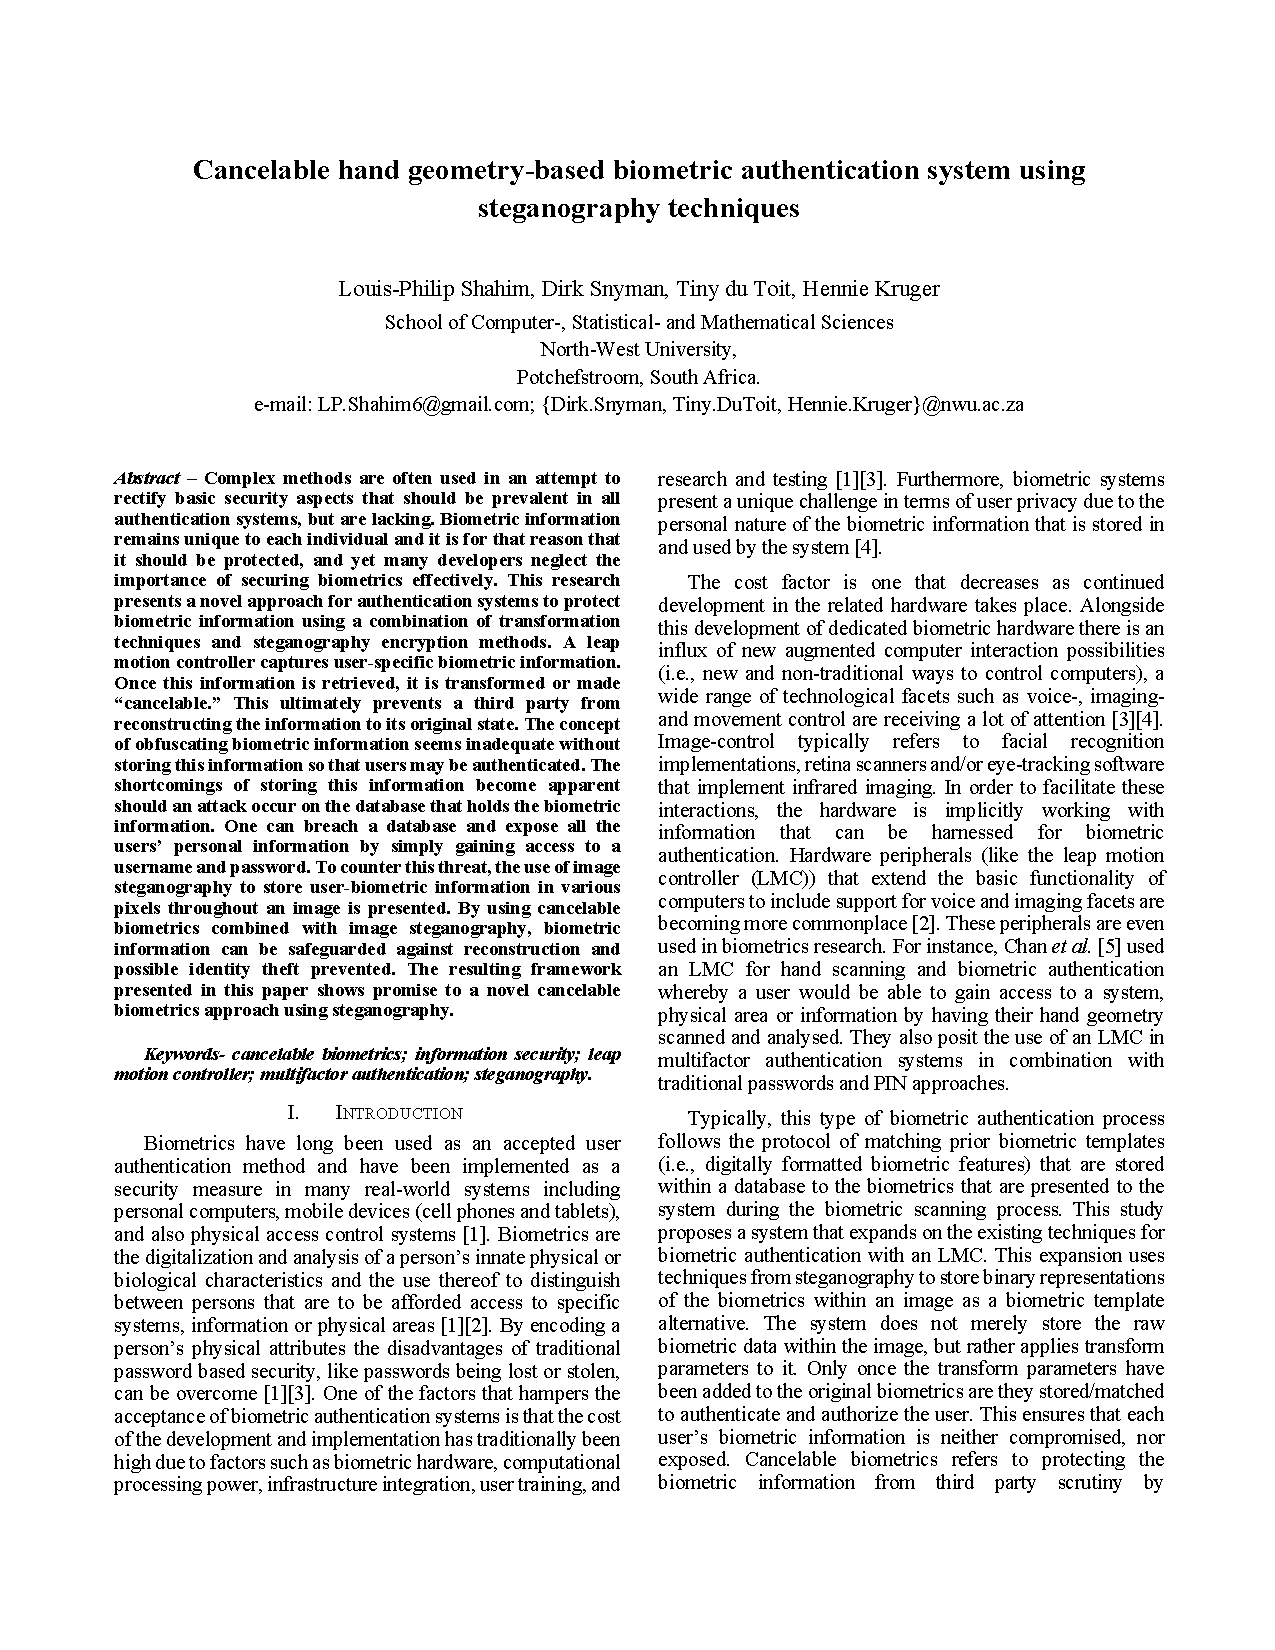
\includepdf[pages=1,scale=.8,pagecommand={\section{Appendix B:} }]{Appendix2/IARIA.pdf}
% \includepdf[pages=2-,pagecommand={}]{Appendix2/IARIA.pdf}

% % %!TEX root = ../thesis.tex
% % ******************************* Thesis Appendix B ********************************

\chapter{Minimum system requirements}
\label{AppendixC}

To successfully use the proposed authentication system that supports the Leap Motion Controller peripheral device, the following minimum system requirements need to be met. 

\begin{enumerate}[label=\roman*.]
    \item Windows 7+ and/or Mac OS X 10.7 +;
    \item AMD Phenom II or Intel Core i3/i5/i7 processor;
    \item 2GB RAM; and a
    \item USB 2.0 port
\end{enumerate}
    


\end{appendices}

% *************************************** Index ********************************
\printthesisindex % If index is present
\end{document}
